% Options for packages loaded elsewhere
\PassOptionsToPackage{unicode}{hyperref}
\PassOptionsToPackage{hyphens}{url}
%
\documentclass[
]{article}
\usepackage{lmodern}
\usepackage{amsmath}
\usepackage{ifxetex,ifluatex}
\ifnum 0\ifxetex 1\fi\ifluatex 1\fi=0 % if pdftex
  \usepackage[T1]{fontenc}
  \usepackage[utf8]{inputenc}
  \usepackage{textcomp} % provide euro and other symbols
  \usepackage{amssymb}
\else % if luatex or xetex
  \usepackage{unicode-math}
  \defaultfontfeatures{Scale=MatchLowercase}
  \defaultfontfeatures[\rmfamily]{Ligatures=TeX,Scale=1}
\fi
% Use upquote if available, for straight quotes in verbatim environments
\IfFileExists{upquote.sty}{\usepackage{upquote}}{}
\IfFileExists{microtype.sty}{% use microtype if available
  \usepackage[]{microtype}
  \UseMicrotypeSet[protrusion]{basicmath} % disable protrusion for tt fonts
}{}
\makeatletter
\@ifundefined{KOMAClassName}{% if non-KOMA class
  \IfFileExists{parskip.sty}{%
    \usepackage{parskip}
  }{% else
    \setlength{\parindent}{0pt}
    \setlength{\parskip}{6pt plus 2pt minus 1pt}}
}{% if KOMA class
  \KOMAoptions{parskip=half}}
\makeatother
\usepackage{xcolor}
\IfFileExists{xurl.sty}{\usepackage{xurl}}{} % add URL line breaks if available
\IfFileExists{bookmark.sty}{\usepackage{bookmark}}{\usepackage{hyperref}}
\hypersetup{
  pdftitle={geodiv Examples},
  pdfauthor={Sydne Record, Annie Smith, Phoebe Zarnetske, Kyla Dahlin, Jennifer Costanza, and Adam Wilson},
  hidelinks,
  pdfcreator={LaTeX via pandoc}}
\urlstyle{same} % disable monospaced font for URLs
\usepackage[margin=1in]{geometry}
\usepackage{color}
\usepackage{fancyvrb}
\newcommand{\VerbBar}{|}
\newcommand{\VERB}{\Verb[commandchars=\\\{\}]}
\DefineVerbatimEnvironment{Highlighting}{Verbatim}{commandchars=\\\{\}}
% Add ',fontsize=\small' for more characters per line
\usepackage{framed}
\definecolor{shadecolor}{RGB}{248,248,248}
\newenvironment{Shaded}{\begin{snugshade}}{\end{snugshade}}
\newcommand{\AlertTok}[1]{\textcolor[rgb]{0.94,0.16,0.16}{#1}}
\newcommand{\AnnotationTok}[1]{\textcolor[rgb]{0.56,0.35,0.01}{\textbf{\textit{#1}}}}
\newcommand{\AttributeTok}[1]{\textcolor[rgb]{0.77,0.63,0.00}{#1}}
\newcommand{\BaseNTok}[1]{\textcolor[rgb]{0.00,0.00,0.81}{#1}}
\newcommand{\BuiltInTok}[1]{#1}
\newcommand{\CharTok}[1]{\textcolor[rgb]{0.31,0.60,0.02}{#1}}
\newcommand{\CommentTok}[1]{\textcolor[rgb]{0.56,0.35,0.01}{\textit{#1}}}
\newcommand{\CommentVarTok}[1]{\textcolor[rgb]{0.56,0.35,0.01}{\textbf{\textit{#1}}}}
\newcommand{\ConstantTok}[1]{\textcolor[rgb]{0.00,0.00,0.00}{#1}}
\newcommand{\ControlFlowTok}[1]{\textcolor[rgb]{0.13,0.29,0.53}{\textbf{#1}}}
\newcommand{\DataTypeTok}[1]{\textcolor[rgb]{0.13,0.29,0.53}{#1}}
\newcommand{\DecValTok}[1]{\textcolor[rgb]{0.00,0.00,0.81}{#1}}
\newcommand{\DocumentationTok}[1]{\textcolor[rgb]{0.56,0.35,0.01}{\textbf{\textit{#1}}}}
\newcommand{\ErrorTok}[1]{\textcolor[rgb]{0.64,0.00,0.00}{\textbf{#1}}}
\newcommand{\ExtensionTok}[1]{#1}
\newcommand{\FloatTok}[1]{\textcolor[rgb]{0.00,0.00,0.81}{#1}}
\newcommand{\FunctionTok}[1]{\textcolor[rgb]{0.00,0.00,0.00}{#1}}
\newcommand{\ImportTok}[1]{#1}
\newcommand{\InformationTok}[1]{\textcolor[rgb]{0.56,0.35,0.01}{\textbf{\textit{#1}}}}
\newcommand{\KeywordTok}[1]{\textcolor[rgb]{0.13,0.29,0.53}{\textbf{#1}}}
\newcommand{\NormalTok}[1]{#1}
\newcommand{\OperatorTok}[1]{\textcolor[rgb]{0.81,0.36,0.00}{\textbf{#1}}}
\newcommand{\OtherTok}[1]{\textcolor[rgb]{0.56,0.35,0.01}{#1}}
\newcommand{\PreprocessorTok}[1]{\textcolor[rgb]{0.56,0.35,0.01}{\textit{#1}}}
\newcommand{\RegionMarkerTok}[1]{#1}
\newcommand{\SpecialCharTok}[1]{\textcolor[rgb]{0.00,0.00,0.00}{#1}}
\newcommand{\SpecialStringTok}[1]{\textcolor[rgb]{0.31,0.60,0.02}{#1}}
\newcommand{\StringTok}[1]{\textcolor[rgb]{0.31,0.60,0.02}{#1}}
\newcommand{\VariableTok}[1]{\textcolor[rgb]{0.00,0.00,0.00}{#1}}
\newcommand{\VerbatimStringTok}[1]{\textcolor[rgb]{0.31,0.60,0.02}{#1}}
\newcommand{\WarningTok}[1]{\textcolor[rgb]{0.56,0.35,0.01}{\textbf{\textit{#1}}}}
\usepackage{graphicx}
\makeatletter
\def\maxwidth{\ifdim\Gin@nat@width>\linewidth\linewidth\else\Gin@nat@width\fi}
\def\maxheight{\ifdim\Gin@nat@height>\textheight\textheight\else\Gin@nat@height\fi}
\makeatother
% Scale images if necessary, so that they will not overflow the page
% margins by default, and it is still possible to overwrite the defaults
% using explicit options in \includegraphics[width, height, ...]{}
\setkeys{Gin}{width=\maxwidth,height=\maxheight,keepaspectratio}
% Set default figure placement to htbp
\makeatletter
\def\fps@figure{htbp}
\makeatother
\setlength{\emergencystretch}{3em} % prevent overfull lines
\providecommand{\tightlist}{%
  \setlength{\itemsep}{0pt}\setlength{\parskip}{0pt}}
\setcounter{secnumdepth}{-\maxdimen} % remove section numbering
\ifluatex
  \usepackage{selnolig}  % disable illegal ligatures
\fi

\title{geodiv Examples}
\author{Sydne Record, Annie Smith, Phoebe Zarnetske, Kyla Dahlin,
Jennifer Costanza, and Adam Wilson}
\date{March 17, 2021}

\begin{document}
\maketitle

\newpage 
\tableofcontents 
\newpage

\hypertarget{install-geodiv}{%
\section{\texorpdfstring{Install
\emph{geodiv}}{Install geodiv}}\label{install-geodiv}}

\emph{geodiv} is an R package that provides methods for calculating
gradient surface metrics for continuous analysis of landscape features.
There are a couple of ways to download and install the \emph{geodiv} R
package. You can install the released version of \emph{geodiv} from CRAN
with:

\begin{Shaded}
\begin{Highlighting}[]
\FunctionTok{install.packages}\NormalTok{(}\StringTok{"geodiv"}\NormalTok{)}
\end{Highlighting}
\end{Shaded}

And the development version from GitHub with:

\begin{Shaded}
\begin{Highlighting}[]
\FunctionTok{install.packages}\NormalTok{(}\StringTok{"devtools"}\NormalTok{)}
\NormalTok{devtools}\SpecialCharTok{::}\FunctionTok{install\_github}\NormalTok{(}\StringTok{"bioXgeo/geodiv"}\NormalTok{)}
\end{Highlighting}
\end{Shaded}

Note that Mac OS users may need to install the development tools here to
get the package to install:

\url{https://cran.r-project.org/bin/macosx/tools/}

To begin, let's load the necessary packages for the examples that
follow.

\begin{Shaded}
\begin{Highlighting}[]
\FunctionTok{library}\NormalTok{(geodiv)}
\FunctionTok{library}\NormalTok{(raster)}
\FunctionTok{library}\NormalTok{(rasterVis)}
\FunctionTok{library}\NormalTok{(mapdata)}
\FunctionTok{library}\NormalTok{(maptools)}
\FunctionTok{library}\NormalTok{(rgeos)}
\FunctionTok{library}\NormalTok{(ggplot2)}
\FunctionTok{library}\NormalTok{(tidyverse)}
\FunctionTok{library}\NormalTok{(parallel)}
\FunctionTok{library}\NormalTok{(sf)}
\FunctionTok{library}\NormalTok{(rasterVis)}
\FunctionTok{library}\NormalTok{(ggmap)}
\FunctionTok{library}\NormalTok{(corrplot)}
\FunctionTok{library}\NormalTok{(gridExtra)}
\FunctionTok{library}\NormalTok{(cowplot)}
\FunctionTok{library}\NormalTok{(factoextra)}
\FunctionTok{library}\NormalTok{(cluster)}
\FunctionTok{library}\NormalTok{(rfigshare)}
\end{Highlighting}
\end{Shaded}

\hypertarget{example-1-simple-workflow-with-landsat-ndvi}{%
\section{Example 1: Simple workflow with Landsat
NDVI}\label{example-1-simple-workflow-with-landsat-ndvi}}

The National Aeronautics and Space Administration (NASA) has been
collecting Earth observing images with Landsat for decades. Normalized
Difference Vegetation Index (NDVI) is a measure of vegetation or
greenness that can be quantified from Landsat images by measuring the
difference between near-infrared and red light, which vegetation
strongly reflects and absorbs, respectively. For this first example, we
generated an NDVI image over a small region in southwestern Oregon using
Google Earth Engine. This image is available as a raster layer available
as an R data object entitled `orforest' when \emph{geodiv} is installed.
Google Earth Engine already has a number of tutorials and sample code
and functions for this step that can be accessed on its site:
earthengine.google.com. There are also several ways in which to access
satellite data from R as well. Given that the focus of this tutorial is
on the use of the \emph{geodiv} R package, we provide these data already
generated in Google Earth Engine.

Let's begin by loading the example data, which is a raster layer called
`orforest'.

\begin{Shaded}
\begin{Highlighting}[]
\CommentTok{\# Load the orforest data into your active session.}
\FunctionTok{data}\NormalTok{(orforest)}
\CommentTok{\# check out the properties of the orforest raster layer.}
\NormalTok{orforest}
\CommentTok{\#\textgreater{} class      : RasterLayer }
\CommentTok{\#\textgreater{} dimensions : 371, 371, 137641  (nrow, ncol, ncell)}
\CommentTok{\#\textgreater{} resolution : 0.0002694946, 0.0002694946  (x, y)}
\CommentTok{\#\textgreater{} extent     : {-}123, {-}122.9, 43.00002, 43.1  (xmin, xmax, ymin, ymax)}
\CommentTok{\#\textgreater{} crs        : +proj=longlat +datum=WGS84 +no\_defs }
\CommentTok{\#\textgreater{} source     : memory}
\CommentTok{\#\textgreater{} names      : summer\_ndvi\_p45\_r30\_2000\_2016\_30m }
\CommentTok{\#\textgreater{} values     : 0.09595944, 0.8357643  (min, max)}
\end{Highlighting}
\end{Shaded}

First, we plot the data without any trends removed.

\begin{Shaded}
\begin{Highlighting}[]
\CommentTok{\# Plot orforest without the trend removed.}
\NormalTok{eviCols }\OtherTok{\textless{}{-}} \FunctionTok{colorRampPalette}\NormalTok{(}\FunctionTok{c}\NormalTok{(}\StringTok{\textquotesingle{}lightyellow1\textquotesingle{}}\NormalTok{, }\StringTok{\textquotesingle{}darkgreen\textquotesingle{}}\NormalTok{))(}\DecValTok{100}\NormalTok{)}
\NormalTok{eviTheme }\OtherTok{\textless{}{-}}\NormalTok{ rasterVis}\SpecialCharTok{::}\FunctionTok{rasterTheme}\NormalTok{(}\AttributeTok{region =}\NormalTok{ eviCols)}
\NormalTok{(orig\_ndvi }\OtherTok{\textless{}{-}}\NormalTok{ rasterVis}\SpecialCharTok{::}\FunctionTok{levelplot}\NormalTok{(orforest, }\AttributeTok{margin =}\NormalTok{ F, }
                                  \AttributeTok{par.settings =}\NormalTok{ eviTheme, }\AttributeTok{xlab =} \StringTok{\textquotesingle{}Longitude\textquotesingle{}}\NormalTok{, }
                                  \AttributeTok{ylab =} \StringTok{\textquotesingle{}Latitude\textquotesingle{}}\NormalTok{, }\AttributeTok{main=}\StringTok{\textquotesingle{}orforest original\textquotesingle{}}\NormalTok{))}
\end{Highlighting}
\end{Shaded}

\includegraphics{geodiv_vignette_files/figure-latex/unnamed-chunk-5-1.pdf}

Use the `remove\_plane' function of \emph{geodiv} to remove the best fit
polynomial plane from the image. This function searches polynomials of
orders 0 - 3 to determine which is has the lowest error relative to the
surface values. To fit a plane with a user-specified polynomial order,
you may use the function `fitplane.'

\begin{Shaded}
\begin{Highlighting}[]
\CommentTok{\# Plot orforest with the trend removed.}
\NormalTok{orfor\_rem }\OtherTok{\textless{}{-}} \FunctionTok{remove\_plane}\NormalTok{(orforest)}
\CommentTok{\#\textgreater{} [1] "Order of polynomial that minimizes errors: 0"}
\NormalTok{(orig\_rem\_plot }\OtherTok{\textless{}{-}}\NormalTok{ rasterVis}\SpecialCharTok{::}\FunctionTok{levelplot}\NormalTok{(orfor\_rem, }\AttributeTok{margin =}\NormalTok{ F, }
                                      \AttributeTok{par.settings =}\NormalTok{ eviTheme, }
                                      \AttributeTok{xlab =} \StringTok{\textquotesingle{}Longitude\textquotesingle{}}\NormalTok{, }\AttributeTok{ylab =} \StringTok{\textquotesingle{}Latitude\textquotesingle{}}\NormalTok{, }
                                      \AttributeTok{main=}\StringTok{\textquotesingle{}orforest trend removed\textquotesingle{}}\NormalTok{))}
\end{Highlighting}
\end{Shaded}

\includegraphics{geodiv_vignette_files/figure-latex/unnamed-chunk-6-1.pdf}

You can also plot the raw satellite image (as opposed to the NDVI
derived from Landsat imagery). To do this, create a Google Maps API key
and copy to the indicated location.

\begin{Shaded}
\begin{Highlighting}[]
\CommentTok{\# Plot the actual satellite image.}
\NormalTok{coords }\OtherTok{\textless{}{-}} \FunctionTok{coordinates}\NormalTok{(orforest)}
\NormalTok{lon }\OtherTok{\textless{}{-}} \FunctionTok{mean}\NormalTok{(coords[, }\DecValTok{1}\NormalTok{], }\AttributeTok{na.rm =} \ConstantTok{TRUE}\NormalTok{)}
\NormalTok{lat }\OtherTok{\textless{}{-}} \FunctionTok{mean}\NormalTok{(coords[, }\DecValTok{2}\NormalTok{], }\AttributeTok{na.rm =} \ConstantTok{TRUE}\NormalTok{)}
\NormalTok{api\_key }\OtherTok{\textless{}{-}} \ConstantTok{NA} \CommentTok{\# ADD AN API KEY HERE}
\end{Highlighting}
\end{Shaded}

Once an API key has been inserted, run the following code to get the
satellite image next to the original NDVI image.

\begin{Shaded}
\begin{Highlighting}[]
\CommentTok{\# Register a Google API key.}
\FunctionTok{register\_google}\NormalTok{(api\_key)}

\CommentTok{\# Get a satellite image at the specified longitude and latitude.}
\NormalTok{img }\OtherTok{\textless{}{-}} \FunctionTok{get\_map}\NormalTok{(}\FunctionTok{c}\NormalTok{(lon, lat), }\AttributeTok{zoom =} \DecValTok{13}\NormalTok{, }\AttributeTok{maptype =} \StringTok{\textquotesingle{}satellite\textquotesingle{}}\NormalTok{, }
               \AttributeTok{source =} \StringTok{"google"}\NormalTok{)}

\CommentTok{\# Create a figure with the satellite image using ggplot.}
\NormalTok{satimg }\OtherTok{\textless{}{-}} \FunctionTok{ggmap}\NormalTok{(img) }\SpecialCharTok{+} \FunctionTok{coord\_fixed}\NormalTok{(}\FloatTok{1.7}\NormalTok{) }\SpecialCharTok{+} \FunctionTok{xlab}\NormalTok{(}\StringTok{\textquotesingle{}Longitude\textquotesingle{}}\NormalTok{) }\SpecialCharTok{+} 
  \FunctionTok{ylab}\NormalTok{(}\StringTok{\textquotesingle{}Latitude\textquotesingle{}}\NormalTok{) }\SpecialCharTok{+}
  \FunctionTok{theme}\NormalTok{(}\AttributeTok{axis.title.x =} \FunctionTok{element\_text}\NormalTok{(}\AttributeTok{size =} \DecValTok{12}\NormalTok{),}
        \AttributeTok{axis.title.y =} \FunctionTok{element\_text}\NormalTok{(}\AttributeTok{size =} \DecValTok{12}\NormalTok{),}
        \AttributeTok{plot.margin =} \FunctionTok{unit}\NormalTok{(}\FunctionTok{c}\NormalTok{(}\DecValTok{0}\NormalTok{, }\DecValTok{0}\NormalTok{, }\DecValTok{0}\NormalTok{, }\DecValTok{0}\NormalTok{), }\StringTok{"cm"}\NormalTok{))}

\CommentTok{\# Plot the satellite image next to the original NDVI image.}
\FunctionTok{plot\_grid}\NormalTok{(satimg, orig\_ndvi, }\AttributeTok{ncol =} \DecValTok{2}\NormalTok{, }\AttributeTok{nrow =} \DecValTok{1}\NormalTok{, }\AttributeTok{scale =} \FunctionTok{c}\NormalTok{(}\FloatTok{0.84}\NormalTok{, }\DecValTok{1}\NormalTok{))}
\end{Highlighting}
\end{Shaded}

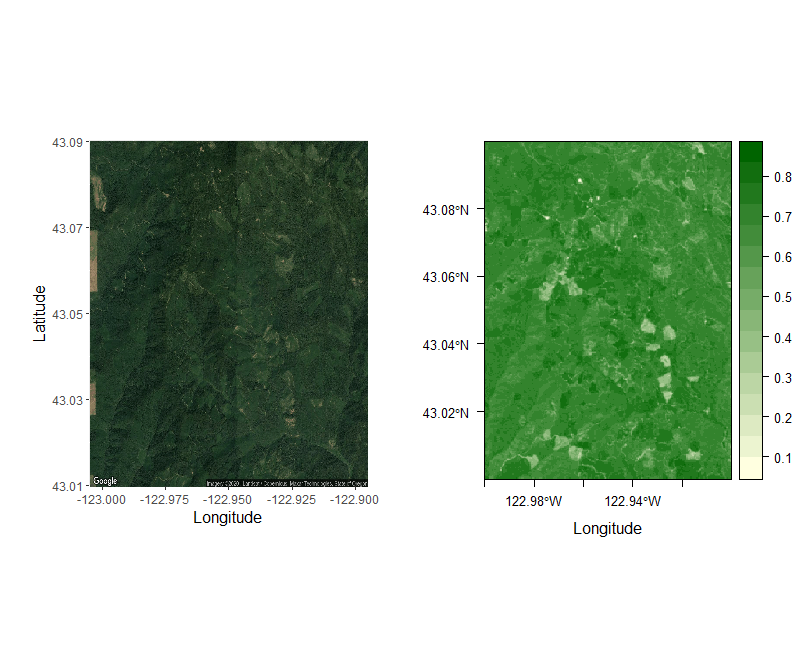
\includegraphics[width=0.9\linewidth]{orig_ndvi_figure}

\hypertarget{calculate-global-surface-gradient-metrics}{%
\subsection{Calculate global surface gradient
metrics}\label{calculate-global-surface-gradient-metrics}}

The simplest use of the \emph{geodiv} package is to apply metrics
globally over an entire image. This returns a measurement of the overall
heterogeneity of the image. The `sa' function calculates the average
roughness of a surface as the absolute deviation of surface heights from
the mean surface height. The `sbi' function calculates the surface
bearing index, which is the ratio of the root mean square roughness (Sq)
to height at 5\% of bearing area (z05). The `std' function calculates
texture direction metrics (i.e., the angle of dominating texture and the
texture direction of the Fourier spectrum image calculated from the
orforest image).

\begin{Shaded}
\begin{Highlighting}[]
\CommentTok{\# Calculate global metrics over the entire orforest image.}
\NormalTok{(sa }\OtherTok{\textless{}{-}} \FunctionTok{sa}\NormalTok{(orforest)) }\CommentTok{\# average roughness}
\CommentTok{\#\textgreater{} [1] 0.04466675}
\NormalTok{(sbi }\OtherTok{\textless{}{-}} \FunctionTok{sbi}\NormalTok{(orforest)) }\CommentTok{\# surface bearing index}
\CommentTok{\#\textgreater{} [1] 0.08557302}
\NormalTok{(std }\OtherTok{\textless{}{-}} \FunctionTok{std}\NormalTok{(orforest, }\AttributeTok{create\_plot =} \ConstantTok{FALSE}\NormalTok{, }\AttributeTok{option =} \DecValTok{1}\NormalTok{))}
\CommentTok{\#\textgreater{} [1] 90}
\end{Highlighting}
\end{Shaded}

\hypertarget{generate-texture-images}{%
\subsection{Generate texture images}\label{generate-texture-images}}

Another common use case is to look at texture images where a spatial
function has been applied locally over focal windows across a landscape.
This functionality is provided through both the `focal\_metrics' and
`texture\_image' functions.

The `texture\_image' function applies metrics in either square or round
windows over the raster. This function tends to be faster than
`focal\_metrics,' but can use more memory when run on Windows. It is
suggested that Windows users use the `focal\_metrics' function instead,
unless they have a computer with a lot of memory.

The `focal\_metrics' function is modified from the `window\_lsm'
function in \emph{landscapemetrics} (Hesselbarth, et al.~2019). Windows
must be rectangular or square, and the `metrics' argument is a list of
functions. The output of this function is a list of rasters.

Note that this step can be somewhat time intensive. For users that would
like to examine the output, but don't want to run this step, the code to
import the rasters is included below.

\begin{Shaded}
\begin{Highlighting}[]
\CommentTok{\# Texture image creation using \textquotesingle{}focal\_metrics\textquotesingle{} function.}
\NormalTok{window }\OtherTok{\textless{}{-}} \FunctionTok{matrix}\NormalTok{(}\DecValTok{1}\NormalTok{, }\AttributeTok{nrow =} \DecValTok{7}\NormalTok{, }\AttributeTok{ncol =} \DecValTok{7}\NormalTok{)}
\FunctionTok{system.time}\NormalTok{(}
\NormalTok{output\_rasters }\OtherTok{\textless{}{-}} \FunctionTok{focal\_metrics}\NormalTok{(orforest, window, }
                                \AttributeTok{metrics =} \FunctionTok{list}\NormalTok{(}\StringTok{\textquotesingle{}sa\textquotesingle{}}\NormalTok{, }\StringTok{\textquotesingle{}sbi\textquotesingle{}}\NormalTok{), }
                                \AttributeTok{progress =} \ConstantTok{TRUE}\NormalTok{)}
\NormalTok{)}

\FunctionTok{print}\NormalTok{(output\_rasters)}

\CommentTok{\# Texture image creation using \textquotesingle{}texture\_image\textquotesingle{} function.}
\NormalTok{metric\_list }\OtherTok{\textless{}{-}} \FunctionTok{c}\NormalTok{(}\StringTok{\textquotesingle{}sa\textquotesingle{}}\NormalTok{, }\StringTok{\textquotesingle{}sbi\textquotesingle{}}\NormalTok{, }\StringTok{\textquotesingle{}std\textquotesingle{}}\NormalTok{)}
\FunctionTok{system.time}\NormalTok{(output\_rasters2 }\OtherTok{\textless{}{-}} \FunctionTok{lapply}\NormalTok{(metric\_list, }\AttributeTok{FUN =} \ControlFlowTok{function}\NormalTok{(m) \{}
  \FunctionTok{texture\_image}\NormalTok{(orforest, }\AttributeTok{window\_type =} \StringTok{\textquotesingle{}square\textquotesingle{}}\NormalTok{, }\AttributeTok{size =} \DecValTok{7}\NormalTok{,}
                                \AttributeTok{in\_meters =} \ConstantTok{FALSE}\NormalTok{, }\AttributeTok{metric =}\NormalTok{ m, }
                                \AttributeTok{parallel =} \ConstantTok{TRUE}\NormalTok{, }\AttributeTok{ncore =} \DecValTok{4}\NormalTok{, }\AttributeTok{nclumps =} \DecValTok{20}\NormalTok{)\}))}
\end{Highlighting}
\end{Shaded}

\begin{Shaded}
\begin{Highlighting}[]
\CommentTok{\# Download rasters from figshare. The list of data returned here will be used}
\CommentTok{\# throughout the vignette.}
\NormalTok{url }\OtherTok{\textless{}{-}} \FunctionTok{fs\_download}\NormalTok{(}\DecValTok{12834896}\NormalTok{, }\AttributeTok{mine =} \ConstantTok{FALSE}\NormalTok{, }\AttributeTok{session =} \ConstantTok{NULL}\NormalTok{)}
\CommentTok{\#\textgreater{} No encoding supplied: defaulting to UTF{-}8.}

\NormalTok{output\_rasters2 }\OtherTok{\textless{}{-}} \FunctionTok{list}\NormalTok{()}
\NormalTok{output\_rasters2[[}\DecValTok{1}\NormalTok{]] }\OtherTok{\textless{}{-}} \FunctionTok{raster}\NormalTok{(url[[}\DecValTok{5}\NormalTok{]])}
\NormalTok{output\_rasters2[[}\DecValTok{2}\NormalTok{]] }\OtherTok{\textless{}{-}} \FunctionTok{raster}\NormalTok{(url[[}\DecValTok{6}\NormalTok{]])}
\NormalTok{output\_rasters2[[}\DecValTok{3}\NormalTok{]] }\OtherTok{\textless{}{-}} \FunctionTok{raster}\NormalTok{(url[[}\DecValTok{7}\NormalTok{]])}
\end{Highlighting}
\end{Shaded}

Plot the texture image rasters.

\begin{Shaded}
\begin{Highlighting}[]
\CommentTok{\# Create list of plots.}
\NormalTok{names }\OtherTok{\textless{}{-}} \FunctionTok{c}\NormalTok{(}\StringTok{\textquotesingle{}Sa\textquotesingle{}}\NormalTok{, }\StringTok{\textquotesingle{}Sbi\textquotesingle{}}\NormalTok{, }\StringTok{\textquotesingle{}Std\textquotesingle{}}\NormalTok{)}
\NormalTok{rast\_list }\OtherTok{\textless{}{-}} \FunctionTok{unlist}\NormalTok{(output\_rasters2) }
\NormalTok{plts }\OtherTok{\textless{}{-}} \FunctionTok{lapply}\NormalTok{(}\FunctionTok{seq}\NormalTok{(}\DecValTok{1}\NormalTok{, }\DecValTok{3}\NormalTok{), }\AttributeTok{FUN =} \ControlFlowTok{function}\NormalTok{(i) \{}
\NormalTok{  rasterVis}\SpecialCharTok{::}\FunctionTok{levelplot}\NormalTok{(rast\_list[[i]], }\AttributeTok{margin =}\NormalTok{ F, }\AttributeTok{par.settings =}\NormalTok{ eviTheme, }
                       \AttributeTok{ylab =} \ConstantTok{NULL}\NormalTok{, }\AttributeTok{xlab =} \ConstantTok{NULL}\NormalTok{, }\AttributeTok{main =}\NormalTok{ names[i])}
\NormalTok{\})}

\CommentTok{\# Arrange plots in the list into a grid.}
\FunctionTok{grid.arrange}\NormalTok{(}\AttributeTok{grobs =}\NormalTok{ plts, }\AttributeTok{nrow =} \DecValTok{2}\NormalTok{)}
\end{Highlighting}
\end{Shaded}

\includegraphics{geodiv_vignette_files/figure-latex/unnamed-chunk-11-1.pdf}

\hypertarget{example-2-applying-all-surface-metrics-across-the-state-of-oregon-usa}{%
\section{Example 2: Applying all surface metrics across the state of
Oregon,
USA}\label{example-2-applying-all-surface-metrics-across-the-state-of-oregon-usa}}

\hypertarget{motivation}{%
\subsection{Motivation}\label{motivation}}

By assessing heterogeneity using a variety of metrics, researchers can
gain a more complete picture of heterogeneity than they would with a
single metric (Dahlin, 2016). To demonstrate the utility of
\emph{geodiv} for this common application, in Example 2 we apply all
surface metric functions to images across Oregon, USA and examine the
patterns of, and relationships among, metrics. We calculate metrics for
both elevation data from the Shuttle Radar Topography Mission (SRTM) and
a commonly-used measure of canopy greenness, Enhanced Vegetation Index
(EVI), from NASA's Moderate Resolution Imaging Spectroradiometer
(MODIS). We then examine the correlations among metrics along a transect
crossing the state, and determine how the metrics cluster using two
methods, hierarchical clustering and Principal Components Analysis
(PCA). This analysis demonstrates the relationships among metrics, with
potential for determining how metrics group and behave with various
input data.

\hypertarget{elevation-and-evi-data}{%
\subsection{Elevation and EVI Data}\label{elevation-and-evi-data}}

Elevation and EVI data that are available to use along with this
vignette were prepared in Google Earth Engine (Gorelick et al., 2017)
and analyzed in R. Void-filled SRTM data (Farr et al., 2007) and
quality-filtered, maximum growing season, MODIS EVI data (Didan, 2015)
were downloaded in Fall 2019. The code chunk below downloads these data
into the current R session from figshare. Again, R may be used to access
satellite data, but we provide previously-prepared data for the purpose
of this analysis.

\begin{Shaded}
\begin{Highlighting}[]
\CommentTok{\# Download data from figshare. }
\NormalTok{elev }\OtherTok{\textless{}{-}} \FunctionTok{raster}\NormalTok{(url[}\DecValTok{4}\NormalTok{])}
\NormalTok{evi }\OtherTok{\textless{}{-}} \FunctionTok{raster}\NormalTok{(url[}\DecValTok{3}\NormalTok{]) }\SpecialCharTok{*} \FloatTok{0.0001}
\end{Highlighting}
\end{Shaded}

Aggregate both datasets to \textasciitilde2km resolution for comparison
between datasets and to reduce computational time.

\begin{Shaded}
\begin{Highlighting}[]
\NormalTok{elev }\OtherTok{\textless{}{-}} \FunctionTok{aggregate}\NormalTok{(elev, }\AttributeTok{fact =} \DecValTok{8}\NormalTok{)}
\NormalTok{evi }\OtherTok{\textless{}{-}} \FunctionTok{aggregate}\NormalTok{(evi, }\AttributeTok{fact =} \DecValTok{8}\NormalTok{)}
\end{Highlighting}
\end{Shaded}

\hypertarget{pre-processing-of-rasters}{%
\subsection{Pre-processing of rasters}\label{pre-processing-of-rasters}}

Begin by masking any values that are outside of the boundaries for the
state of Oregon.

\begin{Shaded}
\begin{Highlighting}[]
\NormalTok{state }\OtherTok{\textless{}{-}}\NormalTok{ maps}\SpecialCharTok{::}\FunctionTok{map}\NormalTok{(}\AttributeTok{database =} \StringTok{\textquotesingle{}state\textquotesingle{}}\NormalTok{, }\AttributeTok{regions =} \StringTok{\textquotesingle{}oregon\textquotesingle{}}\NormalTok{, }
                   \AttributeTok{fill =} \ConstantTok{TRUE}\NormalTok{, }\AttributeTok{plot =} \ConstantTok{FALSE}\NormalTok{)}
\NormalTok{statePoly }\OtherTok{\textless{}{-}} \FunctionTok{map2SpatialPolygons}\NormalTok{(state, }\AttributeTok{IDs =}\NormalTok{ state}\SpecialCharTok{$}\NormalTok{names, }
                                 \AttributeTok{proj4string =} \FunctionTok{CRS}\NormalTok{(}\FunctionTok{proj4string}\NormalTok{(evi)))}
\NormalTok{evi\_masked }\OtherTok{\textless{}{-}} \FunctionTok{mask}\NormalTok{(}\AttributeTok{x =}\NormalTok{ evi, }\AttributeTok{mask =}\NormalTok{ statePoly)}
\NormalTok{elev\_masked }\OtherTok{\textless{}{-}} \FunctionTok{mask}\NormalTok{(}\AttributeTok{x =}\NormalTok{ elev, }\AttributeTok{mask =}\NormalTok{ statePoly)}
\end{Highlighting}
\end{Shaded}

Generate plots to get a sense for the spatial patterns in the data.

\begin{Shaded}
\begin{Highlighting}[]
\CommentTok{\# plot maximum growing season EVI for Oregon}
\NormalTok{rasterVis}\SpecialCharTok{::}\FunctionTok{levelplot}\NormalTok{(evi\_masked, }\AttributeTok{margin =}\NormalTok{ F, }\AttributeTok{par.settings =}\NormalTok{ eviTheme, }
                     \AttributeTok{ylab =} \ConstantTok{NULL}\NormalTok{, }\AttributeTok{xlab =} \ConstantTok{NULL}\NormalTok{, }
                     \AttributeTok{main =} \StringTok{\textquotesingle{}Maximum Growing Season EVI\textquotesingle{}}\NormalTok{)}
\end{Highlighting}
\end{Shaded}

\includegraphics{geodiv_vignette_files/figure-latex/unnamed-chunk-15-1.pdf}

\begin{Shaded}
\begin{Highlighting}[]

\CommentTok{\# plot elevation (in meters) for Oregon}
\NormalTok{elevCols }\OtherTok{\textless{}{-}} \FunctionTok{colorRampPalette}\NormalTok{(}\FunctionTok{c}\NormalTok{(}\StringTok{\textquotesingle{}grey7\textquotesingle{}}\NormalTok{, }\StringTok{\textquotesingle{}grey93\textquotesingle{}}\NormalTok{))(}\DecValTok{100}\NormalTok{)}
\NormalTok{elevTheme }\OtherTok{\textless{}{-}}\NormalTok{ rasterVis}\SpecialCharTok{::}\FunctionTok{rasterTheme}\NormalTok{(}\AttributeTok{region =}\NormalTok{ elevCols)}
\NormalTok{rasterVis}\SpecialCharTok{::}\FunctionTok{levelplot}\NormalTok{(elev\_masked, }\AttributeTok{margin =}\NormalTok{ F, }\AttributeTok{par.settings =}\NormalTok{ elevTheme, }
                     \AttributeTok{ylab =} \ConstantTok{NULL}\NormalTok{, }\AttributeTok{xlab =} \ConstantTok{NULL}\NormalTok{, }\AttributeTok{main =} \StringTok{\textquotesingle{}Elevation (m)\textquotesingle{}}\NormalTok{)}
\end{Highlighting}
\end{Shaded}

\includegraphics{geodiv_vignette_files/figure-latex/unnamed-chunk-15-2.pdf}

Remove any trends in the data with the `remove\_plane' function and take
a look at the plots of the images with the trends removed.

\begin{Shaded}
\begin{Highlighting}[]
\NormalTok{evi\_masked }\OtherTok{\textless{}{-}} \FunctionTok{remove\_plane}\NormalTok{(evi\_masked)}
\CommentTok{\#\textgreater{} [1] "Order of polynomial that minimizes errors: 1"}
\NormalTok{elev\_masked }\OtherTok{\textless{}{-}} \FunctionTok{remove\_plane}\NormalTok{(elev\_masked) }\CommentTok{\# there was no trend}
\CommentTok{\#\textgreater{} [1] "Order of polynomial that minimizes errors: 0"}

\CommentTok{\# plot again to see what the new raster looks like}
\NormalTok{rasterVis}\SpecialCharTok{::}\FunctionTok{levelplot}\NormalTok{(evi\_masked, }\AttributeTok{margin =}\NormalTok{ F, }\AttributeTok{par.settings =}\NormalTok{ eviTheme, }
                     \AttributeTok{ylab =} \ConstantTok{NULL}\NormalTok{, }\AttributeTok{xlab =} \ConstantTok{NULL}\NormalTok{, }\AttributeTok{main =} \StringTok{\textquotesingle{}EVI without Trend\textquotesingle{}}\NormalTok{)}
\end{Highlighting}
\end{Shaded}

\includegraphics{geodiv_vignette_files/figure-latex/unnamed-chunk-16-1.pdf}

\begin{Shaded}
\begin{Highlighting}[]
\NormalTok{rasterVis}\SpecialCharTok{::}\FunctionTok{levelplot}\NormalTok{(elev\_masked, }\AttributeTok{margin =}\NormalTok{ F, }\AttributeTok{par.settings =}\NormalTok{ elevTheme, }
                     \AttributeTok{ylab =} \ConstantTok{NULL}\NormalTok{, }\AttributeTok{xlab =} \ConstantTok{NULL}\NormalTok{, }\AttributeTok{main =} \StringTok{\textquotesingle{}Elevation without Trend\textquotesingle{}}\NormalTok{)}
\end{Highlighting}
\end{Shaded}

\includegraphics{geodiv_vignette_files/figure-latex/unnamed-chunk-16-2.pdf}

\hypertarget{generate-texture-images-of-the-state-of-oregon}{%
\subsection{Generate texture images of the state of
Oregon}\label{generate-texture-images-of-the-state-of-oregon}}

Below we generate a texture image for the state of Oregon using the `sa'
metric for elevation. Note that the following step may take some time.
We provide the output dataframe files along with this vignette for all
metrics included in geodiv for elevation and EVI over
\textasciitilde30km x 30km square moving windows and scaled following
calculation for the subsequent analyses in this vignette.

\begin{Shaded}
\begin{Highlighting}[]
\CommentTok{\# Calculate elevation sa texture image for state of Oregon}
\FunctionTok{system.time}\NormalTok{(outrast }\OtherTok{\textless{}{-}} \FunctionTok{texture\_image}\NormalTok{(elev\_masked, }\AttributeTok{window\_type =} \StringTok{\textquotesingle{}square\textquotesingle{}}\NormalTok{, }\AttributeTok{size =} \DecValTok{7}\NormalTok{, }
                         \AttributeTok{in\_meters =} \ConstantTok{FALSE}\NormalTok{, }\AttributeTok{metric =} \StringTok{\textquotesingle{}sa\textquotesingle{}}\NormalTok{, }\AttributeTok{parallel =} \ConstantTok{TRUE}\NormalTok{,}
                         \AttributeTok{ncores =} \DecValTok{4}\NormalTok{, }\AttributeTok{nclumps =} \DecValTok{20}\NormalTok{))}
\end{Highlighting}
\end{Shaded}

The code below illustrates how to convert the raster generated by the
`texture\_image' function (i.e., outrast) to a dataframe for subsequent
analyses.

\begin{Shaded}
\begin{Highlighting}[]
\CommentTok{\# get raster values}
\NormalTok{vals }\OtherTok{\textless{}{-}}\NormalTok{ outrast[]}

\CommentTok{\# Convert output raster of sa metrics (outrast) to a dataframe for }
\CommentTok{\# easier use in subsequent analyses}
\NormalTok{coords }\OtherTok{\textless{}{-}} \FunctionTok{coordinates}\NormalTok{(outrast)}
\NormalTok{sa\_data\_elev }\OtherTok{\textless{}{-}} \FunctionTok{data.frame}\NormalTok{(}\AttributeTok{x =}\NormalTok{ coords[, }\DecValTok{1}\NormalTok{], }\AttributeTok{y =}\NormalTok{ coords[, }\DecValTok{2}\NormalTok{], }\AttributeTok{v =}\NormalTok{ vals)}
\end{Highlighting}
\end{Shaded}

Generating these data frames can take a while, so we have provided .csv
files for all gradient surface metrics calculated for elevation and EVI
in case you find them useful for working with this vignette. The below
code reads in these provided .csv files by downloading data from
figshare.

\begin{Shaded}
\begin{Highlighting}[]
\CommentTok{\# The list of figshare files was completed above, so grab the appropriate files}
\CommentTok{\# for the csv\textquotesingle{}s of all texture image outputs for Oregon.}
\NormalTok{data\_evi }\OtherTok{\textless{}{-}} \FunctionTok{read.csv}\NormalTok{(url[}\DecValTok{2}\NormalTok{], }\AttributeTok{stringsAsFactors =} \ConstantTok{FALSE}\NormalTok{)}
\NormalTok{data\_elev }\OtherTok{\textless{}{-}} \FunctionTok{read.csv}\NormalTok{(url[}\DecValTok{1}\NormalTok{], }\AttributeTok{stringsAsFactors =} \ConstantTok{FALSE}\NormalTok{)}
\end{Highlighting}
\end{Shaded}

\hypertarget{visualization-of-texture-image-outputs}{%
\subsubsection{Visualization of texture image
outputs}\label{visualization-of-texture-image-outputs}}

Distributions of a few elevation variables:

\begin{Shaded}
\begin{Highlighting}[]
\ControlFlowTok{for}\NormalTok{ (i }\ControlFlowTok{in} \FunctionTok{c}\NormalTok{(}\DecValTok{9}\NormalTok{, }\DecValTok{10}\NormalTok{, }\DecValTok{18}\NormalTok{, }\DecValTok{6}\NormalTok{)) \{}
  \FunctionTok{hist}\NormalTok{(data\_elev[, i], }\AttributeTok{breaks =} \DecValTok{30}\NormalTok{, }\AttributeTok{xlab =} \FunctionTok{names}\NormalTok{(data\_elev)[i], }\AttributeTok{main =} \StringTok{\textquotesingle{}\textquotesingle{}}\NormalTok{)}
\NormalTok{\}}
\end{Highlighting}
\end{Shaded}

\includegraphics{geodiv_vignette_files/figure-latex/unnamed-chunk-20-1.pdf}
\includegraphics{geodiv_vignette_files/figure-latex/unnamed-chunk-20-2.pdf}
\includegraphics{geodiv_vignette_files/figure-latex/unnamed-chunk-20-3.pdf}
\includegraphics{geodiv_vignette_files/figure-latex/unnamed-chunk-20-4.pdf}

The code below visualizes metrics over the entire state in order to
capture different aspects of landscape heterogeneity. Individual metrics
primarily distinguish mountainous versus flat terrain, and managed
versus more natural areas; however, some metrics are difficult to
interpret, or do not show very much variation over the region. The
difficulty of interpreting metrics is a known complicating factor for
their use. Others have addressed this issue and linked metrics with
known ecosystem features or patch metrics (McGarigal et al., 2009;
Kedron et al., 2018).

\begin{Shaded}
\begin{Highlighting}[]
\CommentTok{\# New names for plots}
\NormalTok{plt\_names }\OtherTok{\textless{}{-}} \FunctionTok{data.frame}\NormalTok{(}\AttributeTok{old =} \FunctionTok{names}\NormalTok{(data\_elev)[}\DecValTok{3}\SpecialCharTok{:}\FunctionTok{ncol}\NormalTok{(data\_elev)],}
                        \AttributeTok{new =} \FunctionTok{c}\NormalTok{(}\StringTok{\textquotesingle{}Shw\textquotesingle{}}\NormalTok{, }\StringTok{\textquotesingle{}Srw\textquotesingle{}}\NormalTok{, }\StringTok{\textquotesingle{}Srwi\textquotesingle{}}\NormalTok{, }\StringTok{\textquotesingle{}Std\textquotesingle{}}\NormalTok{, }\StringTok{\textquotesingle{}Stdi\textquotesingle{}}\NormalTok{, }\StringTok{\textquotesingle{}S10z\textquotesingle{}}\NormalTok{,}
                                \StringTok{\textquotesingle{}Sa\textquotesingle{}}\NormalTok{, }\StringTok{\textquotesingle{}Sbi\textquotesingle{}}\NormalTok{, }\StringTok{\textquotesingle{}Sci\textquotesingle{}}\NormalTok{, }\StringTok{\textquotesingle{}Sdc 50{-}55\%\textquotesingle{}}\NormalTok{, }\StringTok{\textquotesingle{}Sdc 80{-}85\%\textquotesingle{}}\NormalTok{,}
                                \StringTok{\textquotesingle{}Sdc 0{-}5\%\textquotesingle{}}\NormalTok{, }\StringTok{\textquotesingle{}Sdq6\textquotesingle{}}\NormalTok{, }\StringTok{\textquotesingle{}Sdr\textquotesingle{}}\NormalTok{, }\StringTok{\textquotesingle{}Sds\textquotesingle{}}\NormalTok{, }\StringTok{\textquotesingle{}Sfd\textquotesingle{}}\NormalTok{, }\StringTok{\textquotesingle{}Sk\textquotesingle{}}\NormalTok{,}
                                \StringTok{\textquotesingle{}Sku\textquotesingle{}}\NormalTok{, }\StringTok{\textquotesingle{}Smean\textquotesingle{}}\NormalTok{, }\StringTok{\textquotesingle{}Sph\textquotesingle{}}\NormalTok{, }\StringTok{\textquotesingle{}Spk\textquotesingle{}}\NormalTok{, }\StringTok{\textquotesingle{}Sq\textquotesingle{}}\NormalTok{, }\StringTok{\textquotesingle{}Ssc\textquotesingle{}}\NormalTok{,}
                                \StringTok{\textquotesingle{}Ssk\textquotesingle{}}\NormalTok{, }\StringTok{\textquotesingle{}Sv\textquotesingle{}}\NormalTok{, }\StringTok{\textquotesingle{}Svi\textquotesingle{}}\NormalTok{, }\StringTok{\textquotesingle{}Svk\textquotesingle{}}\NormalTok{))}

\NormalTok{create\_maps }\OtherTok{\textless{}{-}} \ControlFlowTok{function}\NormalTok{(df, r, theme) \{}
\NormalTok{  maps\_list }\OtherTok{\textless{}{-}} \FunctionTok{list}\NormalTok{()}
  \ControlFlowTok{for}\NormalTok{ (i }\ControlFlowTok{in} \FunctionTok{seq}\NormalTok{(}\DecValTok{3}\NormalTok{, }\FunctionTok{ncol}\NormalTok{(df))) \{}
\NormalTok{    temp }\OtherTok{\textless{}{-}} \FunctionTok{setValues}\NormalTok{(r, df[, i])}
\NormalTok{    temp[}\FunctionTok{is.na}\NormalTok{(r)] }\OtherTok{\textless{}{-}} \ConstantTok{NA}
\NormalTok{    goodname }\OtherTok{\textless{}{-}} \FunctionTok{as.character}\NormalTok{(plt\_names}\SpecialCharTok{$}\NormalTok{new[plt\_names}\SpecialCharTok{$}\NormalTok{old }\SpecialCharTok{==} \FunctionTok{names}\NormalTok{(df)[i]])}
\NormalTok{    maps\_list[[i }\SpecialCharTok{{-}} \DecValTok{2}\NormalTok{]] }\OtherTok{\textless{}{-}}\NormalTok{ rasterVis}\SpecialCharTok{::}\FunctionTok{levelplot}\NormalTok{(temp, }\AttributeTok{margin =}\NormalTok{ F, }
                                              \AttributeTok{par.settings =}\NormalTok{ theme, }
                                              \AttributeTok{ylab =} \ConstantTok{NULL}\NormalTok{, }\AttributeTok{xlab =} \ConstantTok{NULL}\NormalTok{, }
                                              \AttributeTok{main =}\NormalTok{ goodname)}
\NormalTok{    maps\_list[[i }\SpecialCharTok{{-}} \DecValTok{2}\NormalTok{]]}\SpecialCharTok{$}\NormalTok{par.settings}\SpecialCharTok{$}\NormalTok{layout.heights[}
      \FunctionTok{c}\NormalTok{( }\StringTok{\textquotesingle{}bottom.padding\textquotesingle{}}\NormalTok{,}
        \StringTok{\textquotesingle{}top.padding\textquotesingle{}}\NormalTok{,}
        \StringTok{\textquotesingle{}key.sub.padding\textquotesingle{}}\NormalTok{,}
        \StringTok{\textquotesingle{}axis.xlab.padding\textquotesingle{}}\NormalTok{,}
        \StringTok{\textquotesingle{}key.axis.padding\textquotesingle{}}\NormalTok{,}
        \StringTok{\textquotesingle{}main.key.padding\textquotesingle{}}\NormalTok{) ] }\OtherTok{\textless{}{-}} \DecValTok{1}
\NormalTok{    maps\_list[[i }\SpecialCharTok{{-}} \DecValTok{2}\NormalTok{]]}\SpecialCharTok{$}\NormalTok{aspect.fill }\OtherTok{\textless{}{-}} \ConstantTok{TRUE}
    \FunctionTok{names}\NormalTok{(maps\_list)[i }\SpecialCharTok{{-}} \DecValTok{2}\NormalTok{] }\OtherTok{\textless{}{-}}\NormalTok{ goodname}
\NormalTok{  \}}
  \FunctionTok{return}\NormalTok{(maps\_list)}
\NormalTok{\}}

\CommentTok{\# Create plots of all possible surface gradient metrics that geodiv calculates }
\CommentTok{\# for elevation and EVI.}
\NormalTok{elev\_maps }\OtherTok{\textless{}{-}} \FunctionTok{create\_maps}\NormalTok{(data\_elev, elev\_masked, elevTheme)}
\NormalTok{evi\_maps }\OtherTok{\textless{}{-}} \FunctionTok{create\_maps}\NormalTok{(data\_evi, evi\_masked, eviTheme)}

\CommentTok{\# Make sure that order of maps is the same for both EVI and Elevation.}
\NormalTok{new\_order }\OtherTok{\textless{}{-}} \FunctionTok{match}\NormalTok{(plt\_names}\SpecialCharTok{$}\NormalTok{new, }\FunctionTok{names}\NormalTok{(evi\_maps)) }\CommentTok{\# get order according to names table}
\NormalTok{evi\_maps }\OtherTok{\textless{}{-}}\NormalTok{ evi\_maps[new\_order]}

\CommentTok{\# Create map panels (3 each for EVI and elevation).}
\ControlFlowTok{for}\NormalTok{ (l }\ControlFlowTok{in} \FunctionTok{list}\NormalTok{(elev\_maps, evi\_maps)) \{}
  \FunctionTok{grid.arrange}\NormalTok{(}\AttributeTok{grobs =}\NormalTok{ l[}\DecValTok{1}\SpecialCharTok{:}\DecValTok{12}\NormalTok{], }\AttributeTok{nrow =} \DecValTok{4}\NormalTok{, }\AttributeTok{ncol =} \DecValTok{3}\NormalTok{) }\CommentTok{\# 850x800}
  \FunctionTok{grid.arrange}\NormalTok{(}\AttributeTok{grobs =}\NormalTok{ l[}\DecValTok{13}\SpecialCharTok{:}\DecValTok{24}\NormalTok{], }\AttributeTok{nrow =} \DecValTok{4}\NormalTok{, }\AttributeTok{ncol =} \DecValTok{3}\NormalTok{) }\CommentTok{\# 850x800}
  \FunctionTok{grid.arrange}\NormalTok{(}\AttributeTok{grobs =}\NormalTok{ l[}\DecValTok{25}\SpecialCharTok{:}\DecValTok{27}\NormalTok{], }\AttributeTok{nrow =} \DecValTok{4}\NormalTok{, }\AttributeTok{ncol =} \DecValTok{3}\NormalTok{) }\CommentTok{\# 850x800}
\NormalTok{\}}
\end{Highlighting}
\end{Shaded}

\includegraphics{geodiv_vignette_files/figure-latex/unnamed-chunk-21-1.pdf}
\includegraphics{geodiv_vignette_files/figure-latex/unnamed-chunk-21-2.pdf}
\includegraphics{geodiv_vignette_files/figure-latex/unnamed-chunk-21-3.pdf}
\includegraphics{geodiv_vignette_files/figure-latex/unnamed-chunk-21-4.pdf}
\includegraphics{geodiv_vignette_files/figure-latex/unnamed-chunk-21-5.pdf}
\includegraphics{geodiv_vignette_files/figure-latex/unnamed-chunk-21-6.pdf}

\hypertarget{transect-analysis}{%
\subsection{Transect analysis}\label{transect-analysis}}

In the code below, we examine an example of local correlation and
clustering among the surface gradient metrics by extracting values over
a horizontal transect across central Oregon.

First we convert the raw elevation and EVI data from the NASA's SRTM and
MODIS mission, respectively, to a dataframe and add those raw values to
the dataframes for EVI and elevation containing the gradient surface
metrics we've calculated across the state of Oregon.

\begin{Shaded}
\begin{Highlighting}[]
\CommentTok{\# Convert the rasters to dataframe format and add value to dataframe with }
\CommentTok{\# metric values.}
\NormalTok{sp\_df }\OtherTok{\textless{}{-}} \ControlFlowTok{function}\NormalTok{(r, df) \{}
\NormalTok{  pixdf }\OtherTok{\textless{}{-}} \FunctionTok{as.data.frame}\NormalTok{(}\FunctionTok{as}\NormalTok{(r, }\StringTok{"SpatialPixelsDataFrame"}\NormalTok{))}
\NormalTok{  df}\SpecialCharTok{$}\NormalTok{value }\OtherTok{\textless{}{-}}\NormalTok{ pixdf[, }\DecValTok{1}\NormalTok{]}
  \FunctionTok{return}\NormalTok{(df)}
\NormalTok{\}}

\NormalTok{data\_elev }\OtherTok{\textless{}{-}} \FunctionTok{sp\_df}\NormalTok{(elev, data\_elev)}
\NormalTok{data\_evi }\OtherTok{\textless{}{-}} \FunctionTok{sp\_df}\NormalTok{(evi, data\_evi)}
\end{Highlighting}
\end{Shaded}

Now we extract the data along a latitudinal transect going across the
state of Oregon.

\begin{Shaded}
\begin{Highlighting}[]

\CommentTok{\# Create new dataframe of values along a latitudinal transect.}
\NormalTok{get\_transect }\OtherTok{\textless{}{-}} \ControlFlowTok{function}\NormalTok{(r, df) \{}
  \CommentTok{\# Crop raster to center transect (+/{-} 7 pixels North or South).}
\NormalTok{  center\_row }\OtherTok{\textless{}{-}} \FunctionTok{round}\NormalTok{(}\FunctionTok{nrow}\NormalTok{(r) }\SpecialCharTok{/} \DecValTok{2}\NormalTok{)}
\NormalTok{  r\_crop }\OtherTok{\textless{}{-}} \FunctionTok{crop}\NormalTok{(r, }\FunctionTok{extent}\NormalTok{(r, center\_row }\SpecialCharTok{{-}} \DecValTok{7}\NormalTok{, center\_row }\SpecialCharTok{+} \DecValTok{7}\NormalTok{, }\DecValTok{1}\NormalTok{, }\FunctionTok{ncol}\NormalTok{(r)))}
  
  \CommentTok{\# Get 8th latitudinal coordinate (center latitude) from the cropped raster.}
\NormalTok{  central\_y }\OtherTok{\textless{}{-}} \FunctionTok{unique}\NormalTok{(}\FunctionTok{coordinates}\NormalTok{(r\_crop)[, }\DecValTok{2}\NormalTok{])[}\DecValTok{8}\NormalTok{]}
  
  \CommentTok{\# Get the closest latitude in the dataframe to the central raster coordinate.}
\NormalTok{  central\_y }\OtherTok{\textless{}{-}} \FunctionTok{unique}\NormalTok{(df}\SpecialCharTok{$}\NormalTok{y[}\FunctionTok{near}\NormalTok{(df}\SpecialCharTok{$}\NormalTok{y, central\_y, }\FloatTok{0.01}\NormalTok{)])[}\DecValTok{1}\NormalTok{]}

  \CommentTok{\# Extract mean EVI and elevation values by raster column.}
\NormalTok{  r\_means }\OtherTok{\textless{}{-}} \FunctionTok{colMeans}\NormalTok{(}\FunctionTok{as.matrix}\NormalTok{(r\_crop), }\AttributeTok{na.rm =} \ConstantTok{TRUE}\NormalTok{)}

  \CommentTok{\# Now limit the dataframe to the central row across the transect.}
\NormalTok{  transect\_vals }\OtherTok{\textless{}{-}}\NormalTok{ df[df}\SpecialCharTok{$}\NormalTok{y }\SpecialCharTok{==}\NormalTok{ central\_y,]}

  \CommentTok{\# Add column means to dataframe.}
\NormalTok{  transect\_vals}\SpecialCharTok{$}\NormalTok{value }\OtherTok{\textless{}{-}}\NormalTok{ r\_means}
  
  \FunctionTok{return}\NormalTok{(transect\_vals)}
\NormalTok{\}}

\NormalTok{transect\_elev }\OtherTok{\textless{}{-}} \FunctionTok{get\_transect}\NormalTok{(elev, data\_elev)}
\NormalTok{transect\_evi }\OtherTok{\textless{}{-}} \FunctionTok{get\_transect}\NormalTok{(evi, data\_evi)}
\end{Highlighting}
\end{Shaded}

The code below places standardizes all metrics by placing them on the
same scale from 0 - 1.

\begin{Shaded}
\begin{Highlighting}[]
\CommentTok{\# Get all metrics on same scale (0{-}1).}
\NormalTok{scale\_mets }\OtherTok{\textless{}{-}} \ControlFlowTok{function}\NormalTok{(df) \{}
  \ControlFlowTok{for}\NormalTok{ (i }\ControlFlowTok{in} \DecValTok{3}\SpecialCharTok{:}\FunctionTok{ncol}\NormalTok{(df)) \{}
\NormalTok{     df[,i] }\OtherTok{\textless{}{-}}\NormalTok{ (df[, i] }\SpecialCharTok{{-}} \FunctionTok{min}\NormalTok{(df[, i], }\AttributeTok{na.rm =} \ConstantTok{TRUE}\NormalTok{)) }\SpecialCharTok{/} 
\NormalTok{       (}\FunctionTok{max}\NormalTok{(df[, i], }\AttributeTok{na.rm =} \ConstantTok{TRUE}\NormalTok{) }\SpecialCharTok{{-}} \FunctionTok{min}\NormalTok{(df[, i], }\AttributeTok{na.rm =} \ConstantTok{TRUE}\NormalTok{))}
\NormalTok{  \}}
  \FunctionTok{return}\NormalTok{(df)}
\NormalTok{\}}

\NormalTok{transect\_elev }\OtherTok{\textless{}{-}} \FunctionTok{scale\_mets}\NormalTok{(transect\_elev)}
\NormalTok{transect\_evi }\OtherTok{\textless{}{-}} \FunctionTok{scale\_mets}\NormalTok{(transect\_evi)}
\end{Highlighting}
\end{Shaded}

\hypertarget{clustering-analysis-over-transect}{%
\subsubsection{Clustering analysis over
transect}\label{clustering-analysis-over-transect}}

For the transect analysis, we will perform hierarchical clustering on
metric values using the function `eclust' in the package
\emph{factoextra} (Kassambara \& Mundt, 2020). First, some additional
data wrangling is required to prepare the data for the clustering
analysis below.

\begin{Shaded}
\begin{Highlighting}[]

\CommentTok{\# Remove NA values from the metric columns.}
\NormalTok{rm\_nas }\OtherTok{\textless{}{-}} \ControlFlowTok{function}\NormalTok{(df) \{}
  \ControlFlowTok{for}\NormalTok{ (i }\ControlFlowTok{in} \DecValTok{3}\SpecialCharTok{:}\FunctionTok{ncol}\NormalTok{(df)) \{}
\NormalTok{    df }\OtherTok{\textless{}{-}}\NormalTok{ df[}\SpecialCharTok{!}\FunctionTok{is.na}\NormalTok{(df[, i]),]}
\NormalTok{  \}}
  \FunctionTok{return}\NormalTok{(df)}
\NormalTok{\}}

\NormalTok{transect\_elev }\OtherTok{\textless{}{-}} \FunctionTok{rm\_nas}\NormalTok{(transect\_elev)}
\NormalTok{transect\_evi }\OtherTok{\textless{}{-}} \FunctionTok{rm\_nas}\NormalTok{(transect\_evi)}
\end{Highlighting}
\end{Shaded}

The code below performs the clustering analysis on the surface gradient
metrics. We first determine the optimal number of clusters by examining
the gap statistic, and then plot the clustered variables to see the
relationships among them.

\begin{Shaded}
\begin{Highlighting}[]
\DocumentationTok{\#\#\# Plot optimal number of clusters}
\NormalTok{plot\_gap }\OtherTok{\textless{}{-}} \ControlFlowTok{function}\NormalTok{(df) \{}
  \CommentTok{\# enhanced k{-}means clustering}
\NormalTok{  res.km }\OtherTok{\textless{}{-}} \FunctionTok{clusGap}\NormalTok{(}\FunctionTok{t}\NormalTok{(df)[}\DecValTok{3}\SpecialCharTok{:}\NormalTok{(}\FunctionTok{ncol}\NormalTok{(df) }\SpecialCharTok{{-}} \DecValTok{1}\NormalTok{), ], stats}\SpecialCharTok{::}\NormalTok{kmeans, }\AttributeTok{K.max =} \DecValTok{10}\NormalTok{, }
                    \AttributeTok{B =} \DecValTok{100}\NormalTok{, }\AttributeTok{nstart =} \DecValTok{25}\NormalTok{)}
  \CommentTok{\# gap statistic plot}
\NormalTok{  factoextra}\SpecialCharTok{::}\FunctionTok{fviz\_gap\_stat}\NormalTok{(res.km)}
\NormalTok{\}}

\FunctionTok{plot\_gap}\NormalTok{(transect\_evi)}
\end{Highlighting}
\end{Shaded}

\includegraphics{geodiv_vignette_files/figure-latex/unnamed-chunk-26-1.pdf}

\begin{Shaded}
\begin{Highlighting}[]
\FunctionTok{plot\_gap}\NormalTok{(transect\_elev)}
\end{Highlighting}
\end{Shaded}

\includegraphics{geodiv_vignette_files/figure-latex/unnamed-chunk-26-2.pdf}

\begin{Shaded}
\begin{Highlighting}[]

\DocumentationTok{\#\#\# Dendrogram and scatterplot of clusters}
\NormalTok{get\_clusters }\OtherTok{\textless{}{-}} \ControlFlowTok{function}\NormalTok{(df, nclust) \{}
  \CommentTok{\# Enhanced hierarchical clustering using optimal \# of clusters.}
\NormalTok{  res.hc }\OtherTok{\textless{}{-}}\NormalTok{ factoextra}\SpecialCharTok{::}\FunctionTok{eclust}\NormalTok{(}\FunctionTok{t}\NormalTok{(df)[}\DecValTok{3}\SpecialCharTok{:}\NormalTok{(}\FunctionTok{ncol}\NormalTok{(df) }\SpecialCharTok{{-}} \DecValTok{1}\NormalTok{),], }
                                 \StringTok{"hclust"}\NormalTok{, }\AttributeTok{k =}\NormalTok{ nclust)}
  
  \FunctionTok{return}\NormalTok{(res.hc)}
\NormalTok{\}}

\NormalTok{plot\_dendrogram }\OtherTok{\textless{}{-}} \ControlFlowTok{function}\NormalTok{(res.hc, nclust)\{}
  \CommentTok{\# Plot colors}
\NormalTok{  plt\_cols }\OtherTok{\textless{}{-}} \FunctionTok{c}\NormalTok{(}\StringTok{\textquotesingle{}lightgoldenrod1\textquotesingle{}}\NormalTok{, }\StringTok{\textquotesingle{}lightblue\textquotesingle{}}\NormalTok{, }\StringTok{\textquotesingle{}grey\textquotesingle{}}\NormalTok{, }\StringTok{\textquotesingle{}lightsteelblue4\textquotesingle{}}\NormalTok{)}
  
  \CommentTok{\# Dendrogram plot}
  \FunctionTok{fviz\_dend}\NormalTok{(res.hc, }\AttributeTok{rect =} \ConstantTok{FALSE}\NormalTok{, }\AttributeTok{k\_colors =}\NormalTok{ plt\_cols[}\DecValTok{1}\SpecialCharTok{:}\NormalTok{nclust], }
            \AttributeTok{lwd =} \DecValTok{1}\NormalTok{, }\AttributeTok{label\_cols =} \StringTok{\textquotesingle{}black\textquotesingle{}}\NormalTok{, }\AttributeTok{cex =} \FloatTok{0.8}\NormalTok{, }\AttributeTok{main =} \StringTok{""}\NormalTok{, }\AttributeTok{ylab =} \StringTok{""}\NormalTok{, }
            \AttributeTok{type =} \StringTok{\textquotesingle{}rectangle\textquotesingle{}}\NormalTok{, }\AttributeTok{horiz =} \ConstantTok{TRUE}\NormalTok{, }\AttributeTok{labels\_track\_height =} \DecValTok{14}\NormalTok{) }\SpecialCharTok{+} 
    \FunctionTok{theme}\NormalTok{(}\AttributeTok{axis.text.y =} \FunctionTok{element\_blank}\NormalTok{(), }\AttributeTok{axis.ticks =} \FunctionTok{element\_blank}\NormalTok{())}
\NormalTok{\}}

\NormalTok{plot\_scatter }\OtherTok{\textless{}{-}} \ControlFlowTok{function}\NormalTok{(res.hc) \{}
  \CommentTok{\# Scatterplot}
  \FunctionTok{fviz\_cluster}\NormalTok{(res.hc)}
\NormalTok{\}}

\NormalTok{res.hc\_elev }\OtherTok{\textless{}{-}} \FunctionTok{get\_clusters}\NormalTok{(transect\_elev, }\AttributeTok{nclust =} \DecValTok{4}\NormalTok{)}
\NormalTok{res.hc\_evi }\OtherTok{\textless{}{-}} \FunctionTok{get\_clusters}\NormalTok{(transect\_evi, }\AttributeTok{nclust =} \DecValTok{3}\NormalTok{)}

\FunctionTok{plot\_dendrogram}\NormalTok{(res.hc\_elev, }\AttributeTok{nclust =} \DecValTok{4}\NormalTok{)}
\end{Highlighting}
\end{Shaded}

\includegraphics{geodiv_vignette_files/figure-latex/unnamed-chunk-26-3.pdf}

\begin{Shaded}
\begin{Highlighting}[]
\FunctionTok{plot\_dendrogram}\NormalTok{(res.hc\_evi, }\AttributeTok{nclust =} \DecValTok{3}\NormalTok{)}
\end{Highlighting}
\end{Shaded}

\includegraphics{geodiv_vignette_files/figure-latex/unnamed-chunk-26-4.pdf}

\begin{Shaded}
\begin{Highlighting}[]

\FunctionTok{plot\_scatter}\NormalTok{(res.hc\_elev)}
\end{Highlighting}
\end{Shaded}

\includegraphics{geodiv_vignette_files/figure-latex/unnamed-chunk-26-5.pdf}

\begin{Shaded}
\begin{Highlighting}[]
\FunctionTok{plot\_scatter}\NormalTok{(res.hc\_evi)}
\end{Highlighting}
\end{Shaded}

\includegraphics{geodiv_vignette_files/figure-latex/unnamed-chunk-26-6.pdf}

Now we generate plots that show the EVI and elevation surface gradient
metrics along the Oregon state transect.

First, the data have to be gathered into a longer format for this
visualization.

\begin{Shaded}
\begin{Highlighting}[]

\CommentTok{\# Create gathered (long) version of dataframe for the clustering analysis.}
\NormalTok{gather\_data }\OtherTok{\textless{}{-}} \ControlFlowTok{function}\NormalTok{(df) \{}
\NormalTok{  df }\OtherTok{\textless{}{-}}\NormalTok{ df }\SpecialCharTok{\%\textgreater{}\%}\NormalTok{ tidyr}\SpecialCharTok{::}\FunctionTok{gather}\NormalTok{(}\AttributeTok{key =} \StringTok{\textquotesingle{}var\textquotesingle{}}\NormalTok{, }\AttributeTok{value =} \StringTok{\textquotesingle{}value\textquotesingle{}}\NormalTok{, }
                             \FunctionTok{names}\NormalTok{(df[, }\FunctionTok{seq}\NormalTok{(}\DecValTok{3}\NormalTok{, }\FunctionTok{ncol}\NormalTok{(df))]))}
  
  \CommentTok{\# Order variables.}
\NormalTok{  df }\OtherTok{\textless{}{-}}\NormalTok{ df[}\FunctionTok{order}\NormalTok{(df}\SpecialCharTok{$}\NormalTok{var),]}
  
  \FunctionTok{return}\NormalTok{(df)}
\NormalTok{\}}

\NormalTok{gathered\_elev }\OtherTok{\textless{}{-}} \FunctionTok{gather\_data}\NormalTok{(transect\_elev)}
\NormalTok{gathered\_evi }\OtherTok{\textless{}{-}} \FunctionTok{gather\_data}\NormalTok{(transect\_evi)}
\end{Highlighting}
\end{Shaded}

Now we can plot the metrics along the transect, labeling the cluster.

\begin{Shaded}
\begin{Highlighting}[]

\CommentTok{\# Plot metrics along transect, with cluster labeled.}
\NormalTok{plot\_transect\_mets }\OtherTok{\textless{}{-}} \ControlFlowTok{function}\NormalTok{(df, res.hc, varname) \{}
  \CommentTok{\# Map colors to cluster or variable names.}
\NormalTok{  col\_map }\OtherTok{\textless{}{-}} \FunctionTok{c}\NormalTok{(}\StringTok{"1"} \OtherTok{=} \StringTok{"lightgoldenrod1"}\NormalTok{, }\StringTok{"2"} \OtherTok{=} \StringTok{"lightblue"}\NormalTok{, }\StringTok{"3"} \OtherTok{=} \StringTok{"grey"}\NormalTok{,}
               \StringTok{"4"} \OtherTok{=} \StringTok{"lightsteelblue4"}\NormalTok{, }\StringTok{"EVI"} \OtherTok{=} \StringTok{"white"}\NormalTok{, }\StringTok{"Elev"} \OtherTok{=} \StringTok{"white"}\NormalTok{)}
  
  \CommentTok{\# Create a dataframe to match variable names with cluster number.}
\NormalTok{  clust\_df }\OtherTok{\textless{}{-}} \FunctionTok{data.frame}\NormalTok{(}\AttributeTok{var =}\NormalTok{ res.hc}\SpecialCharTok{$}\NormalTok{labels, }\AttributeTok{clust =}\NormalTok{ res.hc}\SpecialCharTok{$}\NormalTok{cluster)}
\NormalTok{  clust\_df }\OtherTok{\textless{}{-}}\NormalTok{ clust\_df[}\FunctionTok{order}\NormalTok{(clust\_df}\SpecialCharTok{$}\NormalTok{clust),]}
  
  \CommentTok{\# Convert var to character.}
\NormalTok{  clust\_df}\SpecialCharTok{$}\NormalTok{var }\OtherTok{\textless{}{-}} \FunctionTok{as.character}\NormalTok{(clust\_df}\SpecialCharTok{$}\NormalTok{var)}
  
  \CommentTok{\# Join cluster number with main dataframe to get cluster labels for plotting.}
\NormalTok{  df }\OtherTok{\textless{}{-}} \FunctionTok{left\_join}\NormalTok{(df, clust\_df, }\AttributeTok{by =} \StringTok{\textquotesingle{}var\textquotesingle{}}\NormalTok{)}
  
  \CommentTok{\# Anything not labeled with a cluster (i.e., the actual value) gets labeled.}
\NormalTok{  df}\SpecialCharTok{$}\NormalTok{clust[}\FunctionTok{is.na}\NormalTok{(df}\SpecialCharTok{$}\NormalTok{clust)] }\OtherTok{\textless{}{-}}\NormalTok{ varname}
  
  \CommentTok{\# Change \textquotesingle{}value\textquotesingle{} label to actual variable name.}
\NormalTok{  df}\SpecialCharTok{$}\NormalTok{var[df}\SpecialCharTok{$}\NormalTok{var }\SpecialCharTok{==} \StringTok{\textquotesingle{}value\textquotesingle{}}\NormalTok{] }\OtherTok{\textless{}{-}}\NormalTok{ varname}
  
  \CommentTok{\# Convert cluster names to factors and match with colors.}
\NormalTok{  df}\SpecialCharTok{$}\NormalTok{clust }\OtherTok{\textless{}{-}} \FunctionTok{as.factor}\NormalTok{(df}\SpecialCharTok{$}\NormalTok{clust) }
\NormalTok{  df}\SpecialCharTok{$}\NormalTok{var }\OtherTok{\textless{}{-}} \FunctionTok{factor}\NormalTok{(df}\SpecialCharTok{$}\NormalTok{var, }\AttributeTok{levels =} \FunctionTok{c}\NormalTok{(clust\_df}\SpecialCharTok{$}\NormalTok{var, varname))}
\NormalTok{  cols\_to\_use }\OtherTok{\textless{}{-}}\NormalTok{ col\_map[}\FunctionTok{names}\NormalTok{(col\_map) }\SpecialCharTok{\%in\%}\NormalTok{ df}\SpecialCharTok{$}\NormalTok{clust]}
  
  \FunctionTok{ggplot}\NormalTok{(df, }\FunctionTok{aes}\NormalTok{(}\AttributeTok{x =}\NormalTok{ x, }\AttributeTok{y =}\NormalTok{ value)) }\SpecialCharTok{+} 
    \FunctionTok{geom\_rect}\NormalTok{(}\FunctionTok{aes}\NormalTok{(}\AttributeTok{xmin =} \SpecialCharTok{{-}}\ConstantTok{Inf}\NormalTok{, }\AttributeTok{xmax =} \ConstantTok{Inf}\NormalTok{, }\AttributeTok{ymin =} \SpecialCharTok{{-}}\ConstantTok{Inf}\NormalTok{, }\AttributeTok{ymax =} \ConstantTok{Inf}\NormalTok{, }
                  \AttributeTok{fill =}\NormalTok{ clust)) }\SpecialCharTok{+}
    \FunctionTok{geom\_line}\NormalTok{(}\AttributeTok{lwd =} \FloatTok{0.7}\NormalTok{) }\SpecialCharTok{+}
    \FunctionTok{xlab}\NormalTok{(}\StringTok{\textquotesingle{}Longitude\textquotesingle{}}\NormalTok{) }\SpecialCharTok{+}
    \FunctionTok{facet\_grid}\NormalTok{(var}\SpecialCharTok{\textasciitilde{}}\NormalTok{., }\AttributeTok{switch =} \StringTok{\textquotesingle{}y\textquotesingle{}}\NormalTok{) }\SpecialCharTok{+}
    \FunctionTok{scale\_fill\_manual}\NormalTok{(}\AttributeTok{values =}\NormalTok{ cols\_to\_use, }\AttributeTok{name =} \StringTok{\textquotesingle{}Cluster\textquotesingle{}}\NormalTok{) }\SpecialCharTok{+}
    \FunctionTok{theme\_bw}\NormalTok{() }\SpecialCharTok{+}
    \FunctionTok{theme}\NormalTok{(}\AttributeTok{axis.title.y =} \FunctionTok{element\_blank}\NormalTok{(),}
          \AttributeTok{axis.text.y =} \FunctionTok{element\_blank}\NormalTok{(),}
          \AttributeTok{strip.text.y.left =} \FunctionTok{element\_text}\NormalTok{(}\AttributeTok{face =} \StringTok{\textquotesingle{}bold\textquotesingle{}}\NormalTok{, }\AttributeTok{size =} \DecValTok{11}\NormalTok{, }\AttributeTok{angle =} \DecValTok{0}\NormalTok{),}
          \AttributeTok{legend.position =} \StringTok{\textquotesingle{}none\textquotesingle{}}\NormalTok{,}
          \AttributeTok{axis.title.x =} \FunctionTok{element\_text}\NormalTok{(}\AttributeTok{face =} \StringTok{\textquotesingle{}bold\textquotesingle{}}\NormalTok{, }\AttributeTok{size =} \DecValTok{11}\NormalTok{))}
\NormalTok{\}}

\FunctionTok{plot\_transect\_mets}\NormalTok{(gathered\_elev, res.hc\_elev, }\StringTok{"Elev"}\NormalTok{)}
\end{Highlighting}
\end{Shaded}

\includegraphics{geodiv_vignette_files/figure-latex/unnamed-chunk-28-1.pdf}

\begin{Shaded}
\begin{Highlighting}[]
\FunctionTok{plot\_transect\_mets}\NormalTok{(gathered\_evi, res.hc\_evi, }\StringTok{"EVI"}\NormalTok{)}
\end{Highlighting}
\end{Shaded}

\includegraphics{geodiv_vignette_files/figure-latex/unnamed-chunk-28-2.pdf}

\hypertarget{summary-of-transect-cluster-analysis}{%
\subsubsection{Summary of transect cluster
analysis}\label{summary-of-transect-cluster-analysis}}

Overall trends along the transect were similar among metrics, with more
variation at smaller intervals. Using hierarchical clustering, we found
four clusters of metrics for elevation, and three for EVI. The metrics
fell into different combinations based on the variable considered
(elevation or EVI). For example, Sdq6 and S10z grouped together for both
variables, but Std and Srw were in the same group for elevation, and
different groups for EVI.

\hypertarget{principal-components-analysis-pca}{%
\subsection{Principal Components Analysis
(PCA)}\label{principal-components-analysis-pca}}

Next, we will determine the statewide elevation and EVI variance
explained by metrics using PCA. First, we need to get the data ready for
the PCA. In the code below, we remove several variables due to their
large number of NA values, caused either by windows containing too few
values, or windows lacking `peaks' or `valleys' (pixels surrounded by
lower or higher values, respectively). After cleaning the data, 21
metrics remain in the analysis.

\begin{Shaded}
\begin{Highlighting}[]
\CommentTok{\# Get data ready for PCA by removing NA values.}
\NormalTok{clean\_data }\OtherTok{\textless{}{-}} \ControlFlowTok{function}\NormalTok{(df) \{}
  \CommentTok{\# Remove columns with very large numbers of NAs.}
\NormalTok{  NAs }\OtherTok{\textless{}{-}} \FunctionTok{sapply}\NormalTok{(df, }\ControlFlowTok{function}\NormalTok{(x) }\FunctionTok{sum}\NormalTok{(}\FunctionTok{is.na}\NormalTok{(x)))}
\NormalTok{  rm\_cols }\OtherTok{\textless{}{-}} \FunctionTok{which}\NormalTok{(NAs }\SpecialCharTok{\textgreater{}=} \DecValTok{20000}\NormalTok{)}
\NormalTok{  df }\OtherTok{\textless{}{-}}\NormalTok{ df[, }\SpecialCharTok{{-}}\NormalTok{rm\_cols]}
  \CommentTok{\# Remove NAs from remaining columns.}
\NormalTok{  df }\OtherTok{\textless{}{-}} \FunctionTok{na.omit}\NormalTok{(df)}
  \FunctionTok{return}\NormalTok{(df)}
\NormalTok{\}}

\NormalTok{data\_elev\_noNA }\OtherTok{\textless{}{-}} \FunctionTok{clean\_data}\NormalTok{(data\_elev)}
\NormalTok{data\_evi\_noNA }\OtherTok{\textless{}{-}} \FunctionTok{clean\_data}\NormalTok{(data\_evi)}
\end{Highlighting}
\end{Shaded}

In the code below, the PCA is performed with the remaining metrics using
the `prcomp' function in the \emph{stats} package.

\begin{Shaded}
\begin{Highlighting}[]
\CommentTok{\# Calculate the principal components.}
\NormalTok{elev\_prc }\OtherTok{\textless{}{-}} \FunctionTok{prcomp}\NormalTok{(data\_elev\_noNA[,}\DecValTok{3}\SpecialCharTok{:}\DecValTok{22}\NormalTok{], }\AttributeTok{center =} \ConstantTok{TRUE}\NormalTok{, }\AttributeTok{scale =} \ConstantTok{TRUE}\NormalTok{)}
\NormalTok{evi\_prc }\OtherTok{\textless{}{-}} \FunctionTok{prcomp}\NormalTok{(data\_evi\_noNA[,}\DecValTok{3}\SpecialCharTok{:}\DecValTok{22}\NormalTok{], }\AttributeTok{center =} \ConstantTok{TRUE}\NormalTok{, }\AttributeTok{scale =} \ConstantTok{TRUE}\NormalTok{)}
\FunctionTok{summary}\NormalTok{(elev\_prc)}
\CommentTok{\#\textgreater{} Importance of components:}
\CommentTok{\#\textgreater{}                           PC1    PC2    PC3     PC4     PC5     PC6     PC7}
\CommentTok{\#\textgreater{} Standard deviation     2.3592 1.7964 1.5836 1.28897 1.12823 1.02005 0.99978}
\CommentTok{\#\textgreater{} Proportion of Variance 0.2783 0.1613 0.1254 0.08307 0.06365 0.05203 0.04998}
\CommentTok{\#\textgreater{} Cumulative Proportion  0.2783 0.4396 0.5650 0.64810 0.71174 0.76377 0.81374}
\CommentTok{\#\textgreater{}                            PC8     PC9    PC10    PC11    PC12    PC13    PC14}
\CommentTok{\#\textgreater{} Standard deviation     0.91966 0.79134 0.72898 0.60892 0.58858 0.52619 0.50061}
\CommentTok{\#\textgreater{} Proportion of Variance 0.04229 0.03131 0.02657 0.01854 0.01732 0.01384 0.01253}
\CommentTok{\#\textgreater{} Cumulative Proportion  0.85603 0.88734 0.91391 0.93245 0.94978 0.96362 0.97615}
\CommentTok{\#\textgreater{}                           PC15    PC16    PC17    PC18    PC19    PC20}
\CommentTok{\#\textgreater{} Standard deviation     0.42315 0.34368 0.29564 0.27348 0.11043 0.07380}
\CommentTok{\#\textgreater{} Proportion of Variance 0.00895 0.00591 0.00437 0.00374 0.00061 0.00027}
\CommentTok{\#\textgreater{} Cumulative Proportion  0.98510 0.99101 0.99538 0.99912 0.99973 1.00000}
\FunctionTok{summary}\NormalTok{(evi\_prc)}
\CommentTok{\#\textgreater{} Importance of components:}
\CommentTok{\#\textgreater{}                           PC1    PC2     PC3     PC4     PC5     PC6     PC7}
\CommentTok{\#\textgreater{} Standard deviation     2.5246 1.9870 1.37645 1.25486 1.09009 0.99925 0.96783}
\CommentTok{\#\textgreater{} Proportion of Variance 0.3187 0.1974 0.09473 0.07873 0.05941 0.04992 0.04683}
\CommentTok{\#\textgreater{} Cumulative Proportion  0.3187 0.5161 0.61081 0.68955 0.74896 0.79889 0.84572}
\CommentTok{\#\textgreater{}                            PC8     PC9    PC10    PC11    PC12    PC13    PC14}
\CommentTok{\#\textgreater{} Standard deviation     0.82448 0.79386 0.70303 0.53013 0.50317 0.47567 0.40850}
\CommentTok{\#\textgreater{} Proportion of Variance 0.03399 0.03151 0.02471 0.01405 0.01266 0.01131 0.00834}
\CommentTok{\#\textgreater{} Cumulative Proportion  0.87971 0.91122 0.93593 0.94998 0.96264 0.97396 0.98230}
\CommentTok{\#\textgreater{}                           PC15    PC16   PC17   PC18    PC19    PC20}
\CommentTok{\#\textgreater{} Standard deviation     0.38320 0.30381 0.2531 0.1547 0.14751 0.07128}
\CommentTok{\#\textgreater{} Proportion of Variance 0.00734 0.00461 0.0032 0.0012 0.00109 0.00025}
\CommentTok{\#\textgreater{} Cumulative Proportion  0.98964 0.99426 0.9975 0.9987 0.99975 1.00000}
\end{Highlighting}
\end{Shaded}

Now let's look at some diagnostic plots for the principal components.
Scree plots indicate the importance of the principal components with a
broken stick criterion. The point at which the scree plot curve crosses
the broken stick model distribution, which we will plot in red, is
considered to indicate the maximum number of components to retain.

\begin{Shaded}
\begin{Highlighting}[]
\CommentTok{\# Take a look at the components using a screeplot.}
\NormalTok{plot\_scree }\OtherTok{\textless{}{-}} \ControlFlowTok{function}\NormalTok{(pc\_dat) \{}
  \FunctionTok{screeplot}\NormalTok{(pc\_dat, }\AttributeTok{type =} \StringTok{"l"}\NormalTok{, }\AttributeTok{npcs =} \DecValTok{15}\NormalTok{, }
            \AttributeTok{main =} \StringTok{"Screeplot of the first 10 PCs"}\NormalTok{)}
  \FunctionTok{abline}\NormalTok{(}\AttributeTok{h =} \DecValTok{1}\NormalTok{, }\AttributeTok{col =} \StringTok{"red"}\NormalTok{, }\AttributeTok{lty =} \DecValTok{5}\NormalTok{)}
  \FunctionTok{legend}\NormalTok{(}\StringTok{"topright"}\NormalTok{, }\AttributeTok{legend =} \FunctionTok{c}\NormalTok{(}\StringTok{"Eigenvalue = 1"}\NormalTok{),}
         \AttributeTok{col =} \FunctionTok{c}\NormalTok{(}\StringTok{"red"}\NormalTok{), }\AttributeTok{lty =} \DecValTok{5}\NormalTok{, }\AttributeTok{cex =} \FloatTok{0.6}\NormalTok{)}
\NormalTok{\}}

\FunctionTok{plot\_scree}\NormalTok{(elev\_prc)}
\end{Highlighting}
\end{Shaded}

\includegraphics{geodiv_vignette_files/figure-latex/unnamed-chunk-31-1.pdf}

\begin{Shaded}
\begin{Highlighting}[]
\FunctionTok{plot\_scree}\NormalTok{(evi\_prc)}
\end{Highlighting}
\end{Shaded}

\includegraphics{geodiv_vignette_files/figure-latex/unnamed-chunk-31-2.pdf}

We can also take a look at the components for elevation and EVI to see
how much variance the surface metrics explain with cumulative variance
plots.

\begin{Shaded}
\begin{Highlighting}[]
\CommentTok{\# Look at how much variance is explained using a cumulative variance plot.}
\NormalTok{plot\_cvar }\OtherTok{\textless{}{-}} \ControlFlowTok{function}\NormalTok{(pc\_dat) \{}
  \CommentTok{\# Get cumulative variance explained.}
\NormalTok{  cumpro }\OtherTok{\textless{}{-}} \FunctionTok{summary}\NormalTok{(pc\_dat)}\SpecialCharTok{$}\NormalTok{importance[}\DecValTok{3}\NormalTok{, ][}\DecValTok{1}\SpecialCharTok{:}\DecValTok{16}\NormalTok{]}
  
  \CommentTok{\# Create plot of cumulative variance, marking the 5th component as the cutoff.}
  \FunctionTok{plot}\NormalTok{(cumpro, }\AttributeTok{xlab =} \StringTok{"PC \#"}\NormalTok{, }\AttributeTok{ylab =} \StringTok{"Amount of explained variance"}\NormalTok{, }
       \AttributeTok{main =} \StringTok{"Cumulative variance plot"}\NormalTok{)}
  \FunctionTok{abline}\NormalTok{(}\AttributeTok{v =} \DecValTok{5}\NormalTok{, }\AttributeTok{col =} \StringTok{"blue"}\NormalTok{, }\AttributeTok{lty =} \DecValTok{5}\NormalTok{)}
  \FunctionTok{abline}\NormalTok{(}\AttributeTok{h =}\NormalTok{ cumpro[}\DecValTok{5}\NormalTok{], }\AttributeTok{col =} \StringTok{"blue"}\NormalTok{, }\AttributeTok{lty =} \DecValTok{5}\NormalTok{)}
  \FunctionTok{legend}\NormalTok{(}\StringTok{"topleft"}\NormalTok{, }\AttributeTok{legend =} \FunctionTok{c}\NormalTok{(}\StringTok{"Cut{-}off @ PC5"}\NormalTok{),}
         \AttributeTok{col =} \FunctionTok{c}\NormalTok{(}\StringTok{"blue"}\NormalTok{), }\AttributeTok{lty =} \DecValTok{5}\NormalTok{, }\AttributeTok{cex =} \FloatTok{0.6}\NormalTok{)}
\NormalTok{\}}

\FunctionTok{plot\_cvar}\NormalTok{(elev\_prc)}
\end{Highlighting}
\end{Shaded}

\includegraphics{geodiv_vignette_files/figure-latex/unnamed-chunk-32-1.pdf}

\begin{Shaded}
\begin{Highlighting}[]
\FunctionTok{plot\_cvar}\NormalTok{(evi\_prc)}
\end{Highlighting}
\end{Shaded}

\includegraphics{geodiv_vignette_files/figure-latex/unnamed-chunk-32-2.pdf}

For both elevation and EVI, the first 5 principal components explained
\textgreater70\% of the variation. Now, let's plot the first components
for elevation.

\begin{Shaded}
\begin{Highlighting}[]

\CommentTok{\# Create scatterplots to look at relationships among principal components.}
\FunctionTok{plot}\NormalTok{(elev\_prc}\SpecialCharTok{$}\NormalTok{x[, }\DecValTok{1}\NormalTok{], elev\_prc}\SpecialCharTok{$}\NormalTok{x[, }\DecValTok{2}\NormalTok{], }\AttributeTok{xlab =} \StringTok{"PC1 (27.83\%)"}\NormalTok{, }
     \AttributeTok{ylab =} \StringTok{"PC2 (16.13\%)"}\NormalTok{, }\AttributeTok{main =} \StringTok{"PC1 / PC2 {-} plot"}\NormalTok{)}
\end{Highlighting}
\end{Shaded}

\includegraphics{geodiv_vignette_files/figure-latex/unnamed-chunk-33-1.pdf}

\begin{Shaded}
\begin{Highlighting}[]
\FunctionTok{plot}\NormalTok{(elev\_prc}\SpecialCharTok{$}\NormalTok{x[, }\DecValTok{1}\NormalTok{], elev\_prc}\SpecialCharTok{$}\NormalTok{x[, }\DecValTok{3}\NormalTok{], }\AttributeTok{xlab =} \StringTok{"PC1 (27.83\%)"}\NormalTok{, }
     \AttributeTok{ylab =} \StringTok{"PC3 (12.54\%)"}\NormalTok{, }\AttributeTok{main =} \StringTok{"PC1 / PC3 {-} plot"}\NormalTok{)}
\end{Highlighting}
\end{Shaded}

\includegraphics{geodiv_vignette_files/figure-latex/unnamed-chunk-33-2.pdf}

\begin{Shaded}
\begin{Highlighting}[]
\FunctionTok{plot}\NormalTok{(elev\_prc}\SpecialCharTok{$}\NormalTok{x[, }\DecValTok{2}\NormalTok{], elev\_prc}\SpecialCharTok{$}\NormalTok{x[, }\DecValTok{3}\NormalTok{], }\AttributeTok{xlab =} \StringTok{"PC2 (16.13\%)"}\NormalTok{, }
     \AttributeTok{ylab =} \StringTok{"PC3 (12.54\%)"}\NormalTok{, }\AttributeTok{main =} \StringTok{"PC2 / PC3 {-} plot"}\NormalTok{)}
\end{Highlighting}
\end{Shaded}

\includegraphics{geodiv_vignette_files/figure-latex/unnamed-chunk-33-3.pdf}

In the code below, we map the components to see if there are any spatial
patterns readily identifiable.

\begin{Shaded}
\begin{Highlighting}[]

\CommentTok{\# Map components across state.}
\NormalTok{map\_comps }\OtherTok{\textless{}{-}} \ControlFlowTok{function}\NormalTok{(pc\_dat, noNA\_df, full\_df, r, theme) \{}
  \CommentTok{\# Add pc values to no{-}NA dataframe.}
  \ControlFlowTok{for}\NormalTok{ (i }\ControlFlowTok{in} \DecValTok{1}\SpecialCharTok{:}\DecValTok{5}\NormalTok{) \{}
\NormalTok{    colname }\OtherTok{\textless{}{-}} \FunctionTok{paste0}\NormalTok{(}\StringTok{\textquotesingle{}prc\textquotesingle{}}\NormalTok{, i)}
\NormalTok{    noNA\_df[, colname] }\OtherTok{\textless{}{-}}\NormalTok{ pc\_dat}\SpecialCharTok{$}\NormalTok{x[, i]}
\NormalTok{  \}}
  
  \CommentTok{\# Add PCA results back to full raster dataframe.}
\NormalTok{  full\_dat }\OtherTok{\textless{}{-}}\NormalTok{ full\_df }\SpecialCharTok{\%\textgreater{}\%} \FunctionTok{left\_join}\NormalTok{(noNA\_df)}
  \CommentTok{\# Cut to only the prc columns.}
\NormalTok{  full\_dat }\OtherTok{\textless{}{-}}\NormalTok{ full\_dat[, }\FunctionTok{grep}\NormalTok{(}\StringTok{\textquotesingle{}prc\textquotesingle{}}\NormalTok{, }\FunctionTok{names}\NormalTok{(full\_dat))]}
  
  \CommentTok{\# Create rasters and maps with principle component values.}
\NormalTok{  out\_maps }\OtherTok{\textless{}{-}} \FunctionTok{list}\NormalTok{()}
  \ControlFlowTok{for}\NormalTok{ (i }\ControlFlowTok{in} \DecValTok{1}\SpecialCharTok{:}\DecValTok{5}\NormalTok{) \{}
\NormalTok{    new\_rast }\OtherTok{\textless{}{-}} \FunctionTok{setValues}\NormalTok{(r, full\_dat[, i])}
\NormalTok{    pc\_map }\OtherTok{\textless{}{-}}\NormalTok{ rasterVis}\SpecialCharTok{::}\FunctionTok{levelplot}\NormalTok{(new\_rast, }\AttributeTok{margin =}\NormalTok{ F, }
                                   \AttributeTok{par.settings =}\NormalTok{ theme, }
                                   \AttributeTok{ylab =} \ConstantTok{NULL}\NormalTok{, }\AttributeTok{xlab =} \ConstantTok{NULL}\NormalTok{, }
                                   \AttributeTok{main =} \FunctionTok{paste0}\NormalTok{(}\StringTok{\textquotesingle{}PC\textquotesingle{}}\NormalTok{, i))}
\NormalTok{    pc\_map}\SpecialCharTok{$}\NormalTok{par.settings}\SpecialCharTok{$}\NormalTok{layout.heights[}\FunctionTok{c}\NormalTok{( }\StringTok{\textquotesingle{}bottom.padding\textquotesingle{}}\NormalTok{,}
                                          \StringTok{\textquotesingle{}top.padding\textquotesingle{}}\NormalTok{,}
                                          \StringTok{\textquotesingle{}key.sub.padding\textquotesingle{}}\NormalTok{,}
                                          \StringTok{\textquotesingle{}axis.xlab.padding\textquotesingle{}}\NormalTok{,}
                                          \StringTok{\textquotesingle{}key.axis.padding\textquotesingle{}}\NormalTok{,}
                                          \StringTok{\textquotesingle{}main.key.padding\textquotesingle{}}\NormalTok{) ] }\OtherTok{\textless{}{-}} \DecValTok{1}
\NormalTok{    pc\_map}\SpecialCharTok{$}\NormalTok{aspect.fill }\OtherTok{\textless{}{-}} \ConstantTok{TRUE}
\NormalTok{    out\_maps[[i]] }\OtherTok{\textless{}{-}}\NormalTok{ pc\_map}
\NormalTok{  \}}
  
  \CommentTok{\# Plot in a grid.}
  \FunctionTok{grid.arrange}\NormalTok{(}\AttributeTok{grobs =}\NormalTok{ out\_maps, }\AttributeTok{nrow =} \DecValTok{2}\NormalTok{, }\AttributeTok{ncol =} \DecValTok{3}\NormalTok{) }
\NormalTok{\}}

\FunctionTok{map\_comps}\NormalTok{(elev\_prc, data\_elev\_noNA, data\_elev, elev, elevTheme)}
\CommentTok{\#\textgreater{} Joining, by = c("x", "y", "std", "s10z", "sa", "sbi", "sci", "sdc05055", "sdc08085", "sdc0005", "sdq6", "sdr", "sds", "sk", "sku", "sph", "spk", "sq", "ssk", "sv", "svi", "svk", "value")}
\end{Highlighting}
\end{Shaded}

\includegraphics{geodiv_vignette_files/figure-latex/unnamed-chunk-34-1.pdf}

\begin{Shaded}
\begin{Highlighting}[]
\FunctionTok{map\_comps}\NormalTok{(evi\_prc, data\_evi\_noNA, data\_evi, evi, eviTheme)}
\CommentTok{\#\textgreater{} Joining, by = c("x", "y", "s10z", "sa", "sbi", "sci", "sdc05055", "sdc08085", "sdc0005", "sdq6", "sdr", "sds", "sk", "sku", "sph", "spk", "sq", "ssk", "std", "sv", "svi", "svk", "value")}
\end{Highlighting}
\end{Shaded}

\includegraphics{geodiv_vignette_files/figure-latex/unnamed-chunk-35-1.pdf}

What are the principal component loadings for elevation?

\begin{Shaded}
\begin{Highlighting}[]

\CommentTok{\# Plot principal component loadings.}
\NormalTok{plot\_loadings }\OtherTok{\textless{}{-}} \ControlFlowTok{function}\NormalTok{(pc\_dat) \{}
  \CommentTok{\# Get rotation for top 5 components.}
\NormalTok{  loadings }\OtherTok{\textless{}{-}}\NormalTok{ pc\_dat}\SpecialCharTok{$}\NormalTok{rotation[, }\DecValTok{1}\SpecialCharTok{:}\DecValTok{5}\NormalTok{]}
  
  \CommentTok{\# Figure out the relative loadings.}
\NormalTok{  aload }\OtherTok{\textless{}{-}} \FunctionTok{abs}\NormalTok{(loadings)}
\NormalTok{  rel }\OtherTok{\textless{}{-}} \FunctionTok{sweep}\NormalTok{(aload, }\DecValTok{2}\NormalTok{, }\FunctionTok{colSums}\NormalTok{(aload), }\StringTok{"/"}\NormalTok{)}
  
  \CommentTok{\# Convert relative loadings to dataframe.}
\NormalTok{  rel }\OtherTok{\textless{}{-}} \FunctionTok{as.data.frame}\NormalTok{(rel)}
  \CommentTok{\# Get good variable names (from dataframe created earlier).}
\NormalTok{  rel}\SpecialCharTok{$}\NormalTok{var }\OtherTok{\textless{}{-}}\NormalTok{ plt\_names}\SpecialCharTok{$}\NormalTok{new[}\FunctionTok{match}\NormalTok{(}\FunctionTok{rownames}\NormalTok{(rel), plt\_names}\SpecialCharTok{$}\NormalTok{old)]}
  
  \CommentTok{\# Create importance plots.}
\NormalTok{  imp\_plts }\OtherTok{\textless{}{-}} \FunctionTok{list}\NormalTok{()}
  \ControlFlowTok{for}\NormalTok{ (i }\ControlFlowTok{in} \DecValTok{1}\SpecialCharTok{:}\DecValTok{5}\NormalTok{) \{}
\NormalTok{    temp }\OtherTok{\textless{}{-}}\NormalTok{ rel}
    \CommentTok{\# Determine whether component loading is postive or negative.}
\NormalTok{    temp}\SpecialCharTok{$}\NormalTok{sign }\OtherTok{\textless{}{-}} \FunctionTok{factor}\NormalTok{(}\FunctionTok{sapply}\NormalTok{(loadings[, i], }\AttributeTok{FUN =} \ControlFlowTok{function}\NormalTok{(x) x }\SpecialCharTok{/} \FunctionTok{abs}\NormalTok{(x)), }
                        \AttributeTok{levels =} \FunctionTok{c}\NormalTok{(}\SpecialCharTok{{-}}\DecValTok{1}\NormalTok{, }\DecValTok{1}\NormalTok{))}
    
    \CommentTok{\# Order loadings by value.}
\NormalTok{    temp }\OtherTok{\textless{}{-}}\NormalTok{ temp[}\FunctionTok{order}\NormalTok{(temp[, i]),]}
    
\NormalTok{    temp}\SpecialCharTok{$}\NormalTok{var }\OtherTok{\textless{}{-}} \FunctionTok{factor}\NormalTok{(temp}\SpecialCharTok{$}\NormalTok{var, }\AttributeTok{levels =}\NormalTok{ temp}\SpecialCharTok{$}\NormalTok{var)}
    
\NormalTok{    temp\_plt }\OtherTok{\textless{}{-}} \FunctionTok{ggplot}\NormalTok{(temp, }\FunctionTok{aes}\NormalTok{(}\AttributeTok{x =}\NormalTok{ temp[, i], }\AttributeTok{y =}\NormalTok{ var)) }\SpecialCharTok{+}
      \FunctionTok{geom\_point}\NormalTok{(}\AttributeTok{size =} \DecValTok{3}\NormalTok{, }\FunctionTok{aes}\NormalTok{(}\AttributeTok{pch =}\NormalTok{ sign)) }\SpecialCharTok{+}
      \FunctionTok{scale\_shape\_manual}\NormalTok{(}\AttributeTok{name =} \FunctionTok{element\_blank}\NormalTok{(),}
                         \AttributeTok{breaks =} \FunctionTok{c}\NormalTok{(}\DecValTok{1}\NormalTok{, }\SpecialCharTok{{-}}\DecValTok{1}\NormalTok{),}
                         \AttributeTok{values =} \FunctionTok{c}\NormalTok{(}\DecValTok{19}\NormalTok{, }\DecValTok{8}\NormalTok{),}
                         \AttributeTok{labels =} \FunctionTok{c}\NormalTok{(}\StringTok{"Positive"}\NormalTok{, }\StringTok{"Negative"}\NormalTok{)) }\SpecialCharTok{+}
      \FunctionTok{xlab}\NormalTok{(}\FunctionTok{paste0}\NormalTok{(}\StringTok{\textquotesingle{}PC\textquotesingle{}}\NormalTok{, i)) }\SpecialCharTok{+}
      \FunctionTok{ylab}\NormalTok{(}\StringTok{\textquotesingle{}Metric\textquotesingle{}}\NormalTok{) }\SpecialCharTok{+}
      \FunctionTok{theme\_bw}\NormalTok{() }\SpecialCharTok{+}
      \FunctionTok{theme}\NormalTok{(}\AttributeTok{panel.grid.minor =} \FunctionTok{element\_blank}\NormalTok{(),}
            \AttributeTok{legend.justification =} \FunctionTok{c}\NormalTok{(}\DecValTok{1}\NormalTok{, }\DecValTok{0}\NormalTok{), }
            \AttributeTok{legend.position =} \FunctionTok{c}\NormalTok{(}\DecValTok{1}\NormalTok{, }\DecValTok{0}\NormalTok{),}
            \AttributeTok{legend.background =} \FunctionTok{element\_blank}\NormalTok{(),}
            \AttributeTok{legend.text =} \FunctionTok{element\_text}\NormalTok{(}\AttributeTok{size =} \DecValTok{12}\NormalTok{),}
            \AttributeTok{axis.title =} \FunctionTok{element\_text}\NormalTok{(}\AttributeTok{size =} \DecValTok{12}\NormalTok{))}
    
\NormalTok{    imp\_plts[[i]] }\OtherTok{\textless{}{-}}\NormalTok{ temp\_plt}
\NormalTok{  \}}
  
  \CommentTok{\# Return grid of first three components.}
  \FunctionTok{grid.arrange}\NormalTok{(}\AttributeTok{grobs =}\NormalTok{ imp\_plts[}\DecValTok{1}\SpecialCharTok{:}\DecValTok{3}\NormalTok{], }\AttributeTok{ncol =} \DecValTok{3}\NormalTok{)}
\NormalTok{\}}

\FunctionTok{plot\_loadings}\NormalTok{(elev\_prc)}
\end{Highlighting}
\end{Shaded}

\includegraphics{geodiv_vignette_files/figure-latex/unnamed-chunk-36-1.pdf}

What are the principal component loadings for EVI?

\begin{Shaded}
\begin{Highlighting}[]
\FunctionTok{plot\_loadings}\NormalTok{(evi\_prc)}
\end{Highlighting}
\end{Shaded}

\includegraphics{geodiv_vignette_files/figure-latex/unnamed-chunk-37-1.pdf}

\hypertarget{summary-of-pca}{%
\subsubsection{Summary of PCA}\label{summary-of-pca}}

Looking at the PCA components and loadings, the first component for both
elevation and EVI described general surface heterogeneity, whereas the
second was related to the shape of the regional value distribution. The
metric groupings observed match previous findings, and the first two
components represent the same groupings (roughness and distribution)
found by McGarigal et al.~(2009).

\hypertarget{overall-summary}{%
\subsection{Overall summary}\label{overall-summary}}

The contrast in metric groupings between the transect hierarchical
clustering analysis and statewide PCA demonstrate that there may be
differences in metric information depending on the landscape size and
scale. As the PCA results were more in line with previous results in the
literature, this suggests that those results show the broader metric
grouping habits. The transect results demonstrate that this grouping
does not always hold across different regions.

\hypertarget{references}{%
\section{References}\label{references}}

\begin{enumerate}
\def\labelenumi{\arabic{enumi})}
\item
  Dahlin, K.M. 2016. Spectral diversity area relationships for assessing
  biodiversity in a wildland--agriculture matrix. Ecological
  applications. 26(8):2758-2768.
\item
  Didan, K., Munoz, A.B., Solano, R., Huete, A. 2015. MODIS vegetation
  index user's guide (MOD13 series). University of Arizona: Vegetation
  Index and Phenology Lab.
\item
  Farr, T.G., Rosen, P.A., Caro, E., Crippen, R., Duren, R., Hensley,
  S., Kobrick, M., Paller, M., Rodriguez, E., Roth, L. and Seal, D.
  2007. The shuttle radar topography mission. Reviews of geophysics.
  45(2).
\item
  Gorelick, N., Hancher, M., Dixon, M., Ilyushchenko, S., Thau, D. and
  Moore, R., 2017. Google Earth Engine: Planetary-scale geospatial
  analysis for everyone. Remote sensing of Environment. 202:18-27.
\item
  Hesselbarth, M.H.K., Sciaini, M., With, K.A., Wiegand, K., Nowosad, J.
  2019. landscapemetrics: an open-source R tool to calculate landscape
  metrics. Ecography 42:1648-1657(ver. 0).
\item
  Kassambara, A. and Mundt, F. (2020). factoextra: Extract and Visualize
  the Results of Multivariate Data Analyses. R package version 1.0.7.
  \url{https://CRAN.R-project.org/package=factoextra}
\item
  Kedron, P.J., Frazier, A.E., Ovando-Montejo, G.A., Wang, J. 2018.
  Surface metrics for landscape ecology: a comparison of landscape
  models across ecoregions and scales. Landscape Ecology.
  33(9):1489-504.
\item
  Hesselbarth, M.H.K., Sciaini, M., With, K.A., Wiegand, K., Nowosad, J.
  2019. landscapemetrics: an open-source R tool to calculate landscape
  metrics. Ecography 42:1648-1657(ver. 0).
\item
  McGarigal, K., Tagil, S., Cushman, SA. 2009. Surface metrics: an
  alternative to patch metrics for the quantification of landscape
  structure. Landscape ecology. 24(3):433-50.
\end{enumerate}

\end{document}
